% BioNetFlux Code Structure Diagram
% To be included in master LaTeX document
%
% Usage: % BioNetFlux Code Structure Diagram
% To be included in master LaTeX document
%
% Usage: % BioNetFlux Code Structure Diagram
% To be included in master LaTeX document
%
% Usage: % BioNetFlux Code Structure Diagram
% To be included in master LaTeX document
%
% Usage: \input{docs/code_structure_diagram}

\begin{figure}[htbp]
\centering
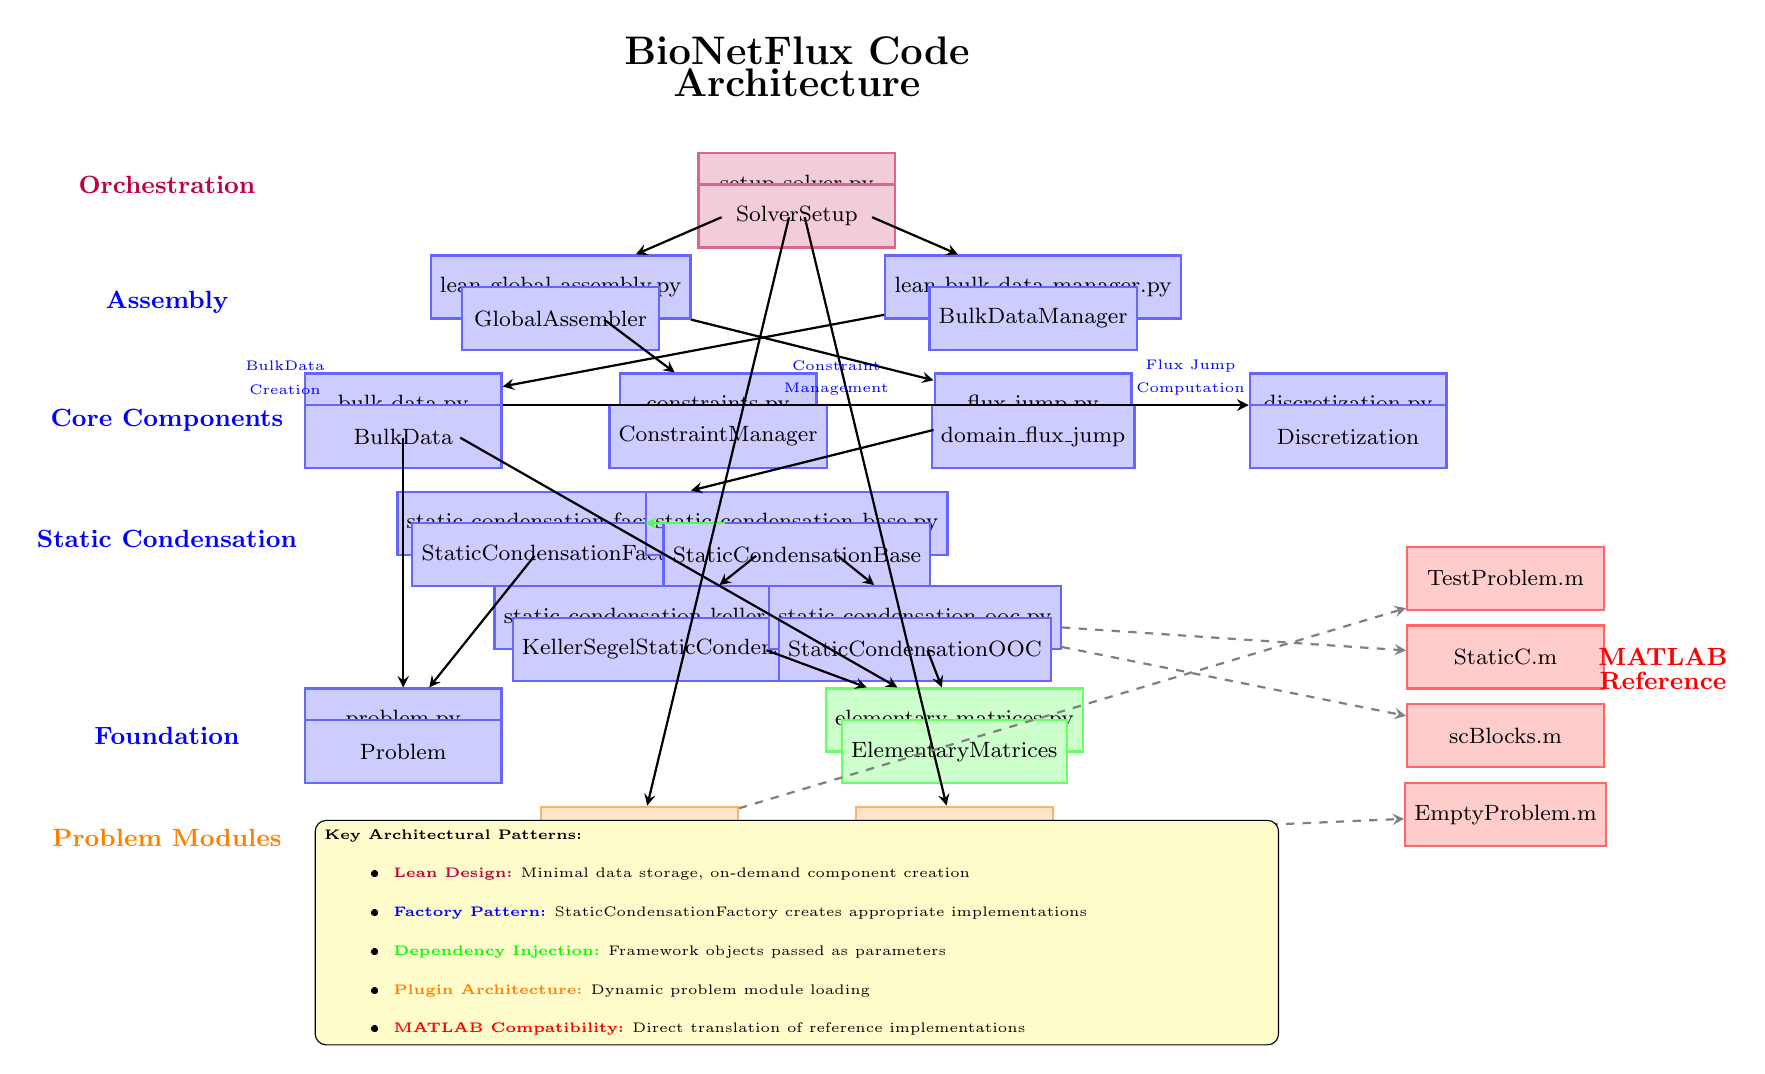
\begin{tikzpicture}[
    % Define styles
    core/.style={rectangle, draw=blue!60, fill=blue!20, thick, minimum width=2.5cm, minimum height=0.8cm, text centered, font=\footnotesize},
    utils/.style={rectangle, draw=green!60, fill=green!20, thick, minimum width=2.5cm, minimum height=0.8cm, text centered, font=\footnotesize},
    problems/.style={rectangle, draw=orange!60, fill=orange!20, thick, minimum width=2.5cm, minimum height=0.8cm, text centered, font=\footnotesize},
    setup/.style={rectangle, draw=purple!60, fill=purple!20, thick, minimum width=2.5cm, minimum height=0.8cm, text centered, font=\footnotesize},
    matlab/.style={rectangle, draw=red!60, fill=red!20, thick, minimum width=2.5cm, minimum height=0.8cm, text centered, font=\footnotesize},
    arrow/.style={->, thick, >=stealth},
    depends/.style={->, dashed, thick, >=stealth, color=gray},
    dataflow/.style={->, thick, >=stealth, color=blue!70},
    factory/.style={->, thick, >=stealth, color=green!70}
]

% Title - Split into two nodes
\node[font=\Large\bfseries] at (0, 10.2) {BioNetFlux Code};
\node[font=\Large\bfseries] at (0, 9.8) {Architecture};

% Layer 1: Setup and Orchestration (Top)
\node[setup] (setup_solver) at (0, 8.5) {setup\_solver.py};
\node[setup] (setup_solver_class) at (0, 8.1) {SolverSetup};

% Layer 2: Core Assembly (Upper Middle)
\node[core] (global_assembly) at (-3, 7.2) {lean\_global\_assembly.py};
\node[core] (global_assembly_class) at (-3, 6.8) {GlobalAssembler};
\node[core] (bulk_manager) at (3, 7.2) {lean\_bulk\_data\_manager.py};
\node[core] (bulk_manager_class) at (3, 6.8) {BulkDataManager};

% Layer 3: Core Components (Middle)
\node[core] (bulk_data) at (-5, 5.7) {bulk\_data.py};
\node[core] (bulk_data_class) at (-5, 5.3) {BulkData};
\node[core] (constraints) at (-1, 5.7) {constraints.py};
\node[core] (constraints_class) at (-1, 5.3) {ConstraintManager};
\node[core] (flux_jump) at (3, 5.7) {flux\_jump.py};
\node[core] (flux_jump_func) at (3, 5.3) {domain\_flux\_jump};
\node[core] (discretization) at (7, 5.7) {discretization.py};
\node[core] (discretization_class) at (7, 5.3) {Discretization};

% Layer 4: Static Condensation (Lower Middle)
\node[core] (sc_factory) at (-3, 4.2) {static\_condensation\_factory.py};
\node[core] (sc_factory_class) at (-3, 3.8) {StaticCondensationFactory};
\node[core] (sc_base) at (0, 4.2) {static\_condensation\_base.py};
\node[core] (sc_base_class) at (0, 3.8) {StaticCondensationBase};
\node[core] (sc_ks) at (-1.5, 3) {static\_condensation\_keller\_segel.py};
\node[core] (sc_ks_class) at (-1.5, 2.6) {KellerSegelStaticCondensation};
\node[core] (sc_ooc) at (1.5, 3) {static\_condensation\_ooc.py};
\node[core] (sc_ooc_class) at (1.5, 2.6) {StaticCondensationOOC};

% Layer 5: Foundation (Bottom)
\node[core] (problem) at (-5, 1.7) {problem.py};
\node[core] (problem_class) at (-5, 1.3) {Problem};
\node[utils] (elementary) at (2, 1.7) {elementary\_matrices.py};
\node[utils] (elementary_class) at (2, 1.3) {ElementaryMatrices};
\node[problems] (test_problem) at (-2, 0.2) {test\_problem2.py};
\node[problems] (double_arc) at (2, 0.2) {double\_arc.py};

% Layer 6: MATLAB Reference (Side)
\node[matlab] (matlab_test) at (9, 3.5) {TestProblem.m};
\node[matlab] (matlab_static) at (9, 2.5) {StaticC.m};
\node[matlab] (matlab_blocks) at (9, 1.5) {scBlocks.m};
\node[matlab] (matlab_empty) at (9, 0.5) {EmptyProblem.m};

% Main orchestration flow
\draw[arrow] (setup_solver) -- (global_assembly);
\draw[arrow] (setup_solver) -- (bulk_manager);

% Assembly dependencies
\draw[arrow] (global_assembly) -- (flux_jump);
\draw[arrow] (global_assembly) -- (constraints);
\draw[arrow] (bulk_manager) -- (bulk_data);

% Core component relationships
\draw[arrow] (flux_jump) -- (sc_factory);
\draw[arrow] (bulk_data) -- (elementary);
\draw[arrow] (bulk_data) -- (discretization);
\draw[arrow] (constraints) -- (discretization);

% Static condensation hierarchy
\draw[factory] (sc_factory) -- (sc_base);
\draw[arrow] (sc_base) -- (sc_ks);
\draw[arrow] (sc_base) -- (sc_ooc);
\draw[arrow] (sc_ks) -- (elementary);
\draw[arrow] (sc_ooc) -- (elementary);

% Problem dependencies
\draw[arrow] (bulk_data) -- (problem);
\draw[arrow] (sc_factory) -- (problem);
\draw[arrow] (setup_solver) -- (test_problem);
\draw[arrow] (setup_solver) -- (double_arc);

% MATLAB reference connections
\draw[depends] (sc_ooc) -- (matlab_static);
\draw[depends] (sc_ooc) -- (matlab_blocks);
\draw[depends] (test_problem) -- (matlab_test);
\draw[depends] (double_arc) -- (matlab_empty);

% Data flow annotations
\node[font=\tiny, color=blue] at (-6.5, 6.2) {BulkData};
\node[font=\tiny, color=blue] at (-6.5, 5.9) {Creation};
\node[font=\tiny, color=blue] at (0.5, 6.2) {Constraint};
\node[font=\tiny, color=blue] at (0.5, 5.9) {Management};
\node[font=\tiny, color=blue] at (5, 6.2) {Flux Jump};
\node[font=\tiny, color=blue] at (5, 5.9) {Computation};

% Layer labels
\node[font=\small\bfseries, color=purple] at (-8, 8.5) {Orchestration};
\node[font=\small\bfseries, color=blue] at (-8, 7) {Assembly};
\node[font=\small\bfseries, color=blue] at (-8, 5.5) {Core Components};
\node[font=\small\bfseries, color=blue] at (-8, 4) {Static Condensation};
\node[font=\small\bfseries, color=blue] at (-8, 1.5) {Foundation};
\node[font=\small\bfseries, color=orange] at (-8, 0.2) {Problem Modules};
\node[font=\small\bfseries, color=red] at (11, 2.5) {MATLAB};
\node[font=\small\bfseries, color=red] at (11, 2.2) {Reference};

% Key architectural patterns
\node[draw, rounded corners, fill=yellow!20, font=\tiny] at (0, -1) {
    \begin{minipage}{12cm}
    \textbf{Key Architectural Patterns:}
    \begin{itemize}
        \item \textcolor{purple}{\textbf{Lean Design:}} Minimal data storage, on-demand component creation
        \item \textcolor{blue}{\textbf{Factory Pattern:}} StaticCondensationFactory creates appropriate implementations
        \item \textcolor{green}{\textbf{Dependency Injection:}} Framework objects passed as parameters
        \item \textcolor{orange}{\textbf{Plugin Architecture:}} Dynamic problem module loading
        \item \textcolor{red}{\textbf{MATLAB Compatibility:}} Direct translation of reference implementations
    \end{itemize}
    \end{minipage}
};

\end{tikzpicture}
\caption[BioNetFlux Code Architecture]{
BioNetFlux code architecture showing the hierarchical structure and dependencies between modules. 
\textcolor{purple}{Purple boxes} represent orchestration layers, 
\textcolor{blue}{blue boxes} represent core computational components, 
\textcolor{green}{green boxes} represent utilities, 
\textcolor{orange}{orange boxes} represent problem-specific modules, and 
\textcolor{red}{red boxes} represent MATLAB reference implementations. 
Solid arrows indicate direct dependencies, dashed arrows indicate reference relationships, 
and colored arrows highlight specific architectural patterns (factory creation, data flow).
The lean design minimizes memory usage through on-demand component creation and parameter-based framework object passing.
}
\label{fig:bionetflux_architecture}
\end{figure}

% Supplementary detailed component diagram
\begin{figure}[htbp]
\centering
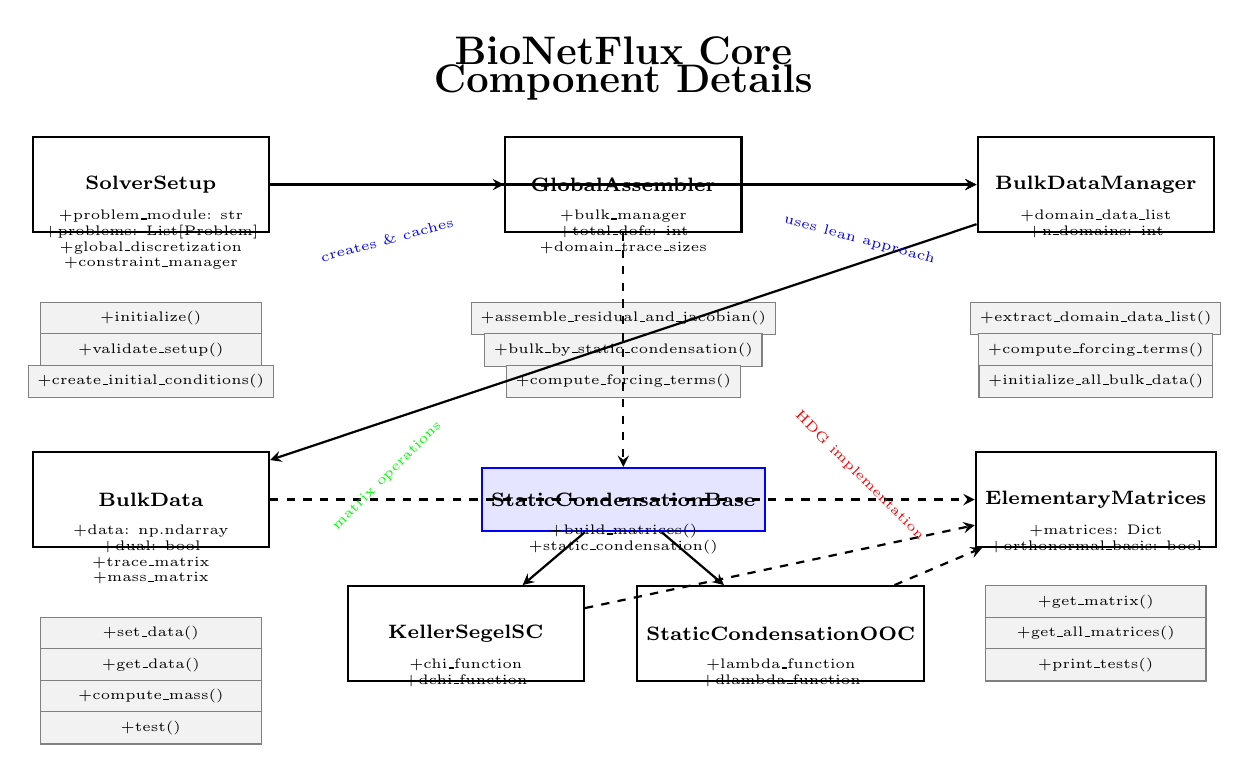
\begin{tikzpicture}[
    % Define styles - Fixed arrow tips
    class/.style={rectangle, draw=black, fill=white, thick, minimum width=3cm, minimum height=1.2cm, text centered, font=\scriptsize},
    method/.style={rectangle, draw=gray, fill=gray!10, minimum width=2.8cm, minimum height=0.4cm, text centered, font=\tiny},
    interface/.style={rectangle, draw=blue, fill=blue!10, thick, minimum width=3cm, minimum height=0.8cm, text centered, font=\scriptsize},
    composition/.style={->, thick, >=stealth},
    inheritance/.style={->, thick, >=stealth},
    usage/.style={->, dashed, thick, >=stealth}
]

% Title
\node[font=\Large\bfseries] at (0, 8.2) {BioNetFlux Core};
\node[font=\Large\bfseries] at (0, 7.8) {Component Details};

% SolverSetup detail
\node[class] (setup_detail) at (-6, 6.5) {
    \textbf{SolverSetup}
};
\node[font=\tiny] at (-6, 6.1) {+problem\_module: str};
\node[font=\tiny] at (-6, 5.9) {+problems: List[Problem]};
\node[font=\tiny] at (-6, 5.7) {+global\_discretization};
\node[font=\tiny] at (-6, 5.5) {+constraint\_manager};

\node[method] (setup_methods) at (-6, 4.8) {+initialize()};
\node[method] (setup_methods2) at (-6, 4.4) {+validate\_setup()};
\node[method] (setup_methods3) at (-6, 4.0) {+create\_initial\_conditions()};

% GlobalAssembler detail
\node[class] (assembler_detail) at (0, 6.5) {
    \textbf{GlobalAssembler}
};
\node[font=\tiny] at (0, 6.1) {+bulk\_manager};
\node[font=\tiny] at (0, 5.9) {+total\_dofs: int};
\node[font=\tiny] at (0, 5.7) {+domain\_trace\_sizes};

\node[method] (assembler_methods) at (0, 4.8) {+assemble\_residual\_and\_jacobian()};
\node[method] (assembler_methods2) at (0, 4.4) {+bulk\_by\_static\_condensation()};
\node[method] (assembler_methods3) at (0, 4.0) {+compute\_forcing\_terms()};

% BulkDataManager detail
\node[class] (manager_detail) at (6, 6.5) {
    \textbf{BulkDataManager}
};
\node[font=\tiny] at (6, 6.1) {+domain\_data\_list};
\node[font=\tiny] at (6, 5.9) {+n\_domains: int};

\node[method] (manager_methods) at (6, 4.8) {+extract\_domain\_data\_list()};
\node[method] (manager_methods2) at (6, 4.4) {+compute\_forcing\_terms()};
\node[method] (manager_methods3) at (6, 4.0) {+initialize\_all\_bulk\_data()};

% BulkData detail
\node[class] (bulk_detail) at (-6, 2.5) {
    \textbf{BulkData}
};
\node[font=\tiny] at (-6, 2.1) {+data: np.ndarray};
\node[font=\tiny] at (-6, 1.9) {+dual: bool};
\node[font=\tiny] at (-6, 1.7) {+trace\_matrix};
\node[font=\tiny] at (-6, 1.5) {+mass\_matrix};

\node[method] (bulk_methods) at (-6, 0.8) {+set\_data()};
\node[method] (bulk_methods2) at (-6, 0.4) {+get\_data()};
\node[method] (bulk_methods3) at (-6, 0.0) {+compute\_mass()};
\node[method] (bulk_methods4) at (-6, -0.4) {+test()};

% StaticCondensation hierarchy
\node[interface] (sc_interface) at (0, 2.5) {
    \textbf{StaticCondensationBase}
};
\node[font=\tiny] at (0, 2.1) {+build\_matrices()};
\node[font=\tiny] at (0, 1.9) {+static\_condensation()};

\node[class] (sc_ks_detail) at (-2, 0.8) {
    \textbf{KellerSegelSC}
};
\node[font=\tiny] at (-2, 0.4) {+chi\_function};
\node[font=\tiny] at (-2, 0.2) {+dchi\_function};

\node[class] (sc_ooc_detail) at (2, 0.8) {
    \textbf{StaticCondensationOOC}
};
\node[font=\tiny] at (2, 0.4) {+lambda\_function};
\node[font=\tiny] at (2, 0.2) {+dlambda\_function};

% ElementaryMatrices detail
\node[class] (elem_detail) at (6, 2.5) {
    \textbf{ElementaryMatrices}
};
\node[font=\tiny] at (6, 2.1) {+matrices: Dict};
\node[font=\tiny] at (6, 1.9) {+orthonormal\_basis: bool};

\node[method] (elem_methods) at (6, 1.2) {+get\_matrix()};
\node[method] (elem_methods2) at (6, 0.8) {+get\_all\_matrices()};
\node[method] (elem_methods3) at (6, 0.4) {+print\_tests()};

% Relationships - Using stealth arrow tips for all
\draw[composition] (setup_detail) -- (assembler_detail);
\draw[composition] (setup_detail) -- (manager_detail);
\draw[composition] (assembler_detail) -- (manager_detail);
\draw[composition] (manager_detail) -- (bulk_detail);
\draw[usage] (assembler_detail) -- (sc_interface);
\draw[inheritance] (sc_interface) -- (sc_ks_detail);
\draw[inheritance] (sc_interface) -- (sc_ooc_detail);
\draw[usage] (bulk_detail) -- (elem_detail);
\draw[usage] (sc_ks_detail) -- (elem_detail);
\draw[usage] (sc_ooc_detail) -- (elem_detail);

% Data flow indicators
\node[font=\tiny, color=blue, rotate=15] at (-3, 5.8) {creates \& caches};
\node[font=\tiny, color=blue, rotate=-15] at (3, 5.8) {uses lean approach};
\node[font=\tiny, color=green, rotate=45] at (-3, 2.8) {matrix operations};
\node[font=\tiny, color=red, rotate=-45] at (3, 2.8) {HDG implementation};

\end{tikzpicture}
\caption[BioNetFlux Component Details]{
Detailed view of key BioNetFlux components showing class structures, main attributes, and key methods. 
Solid arrows indicate composition and inheritance relationships, 
and dashed arrows represent usage dependencies. 
The diagram emphasizes the lean design pattern where components are created on-demand and cached for efficiency.
}
\label{fig:bionetflux_components}
\end{figure}

% Data flow diagram
\begin{figure}[htbp]
\centering
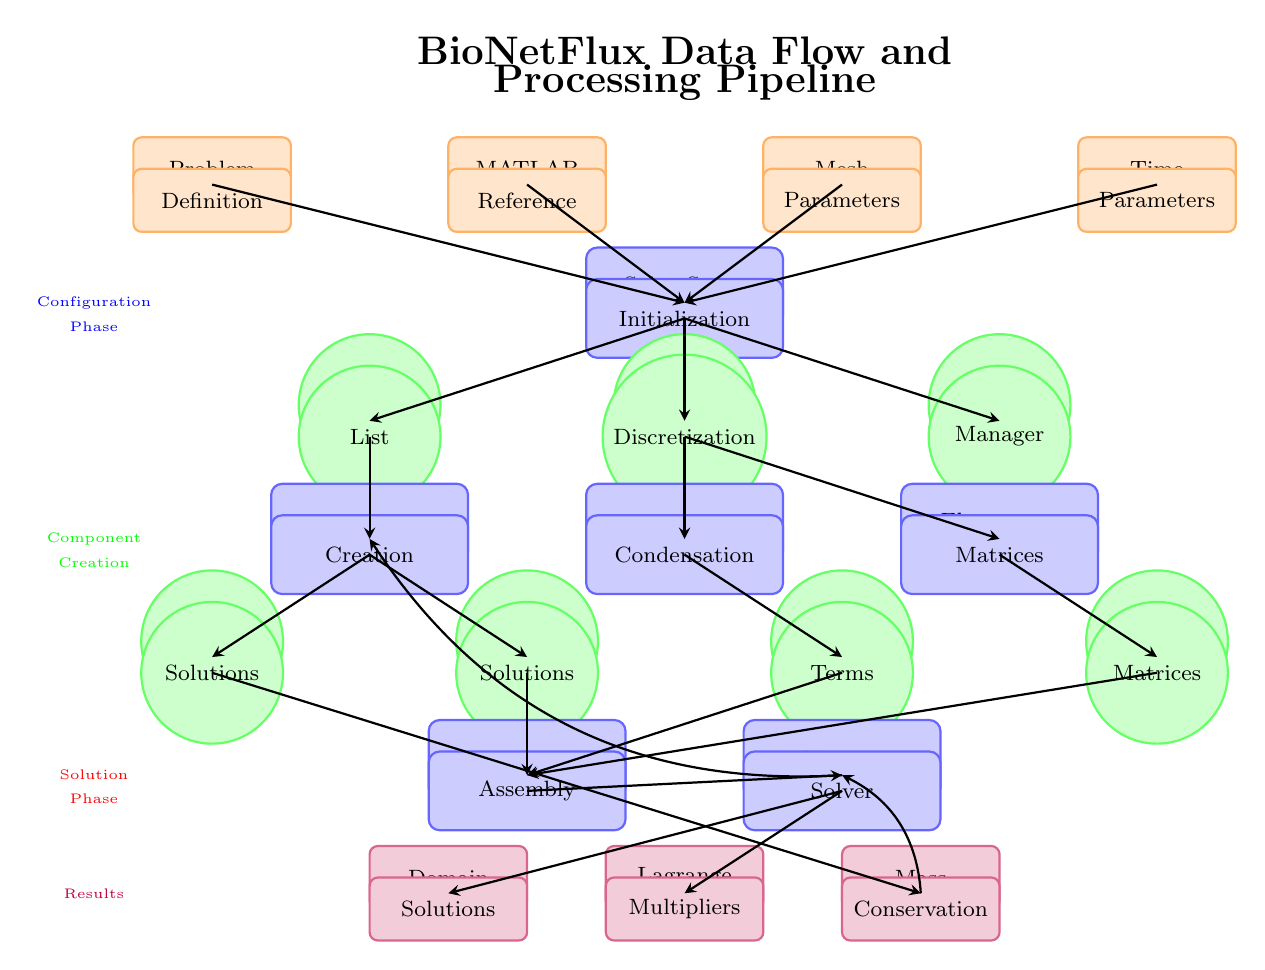
\begin{tikzpicture}[
    % Define styles - Fixed shapes using basic rectangles and circles
    process/.style={rectangle, rounded corners, draw=blue!60, fill=blue!20, thick, minimum width=2.5cm, minimum height=1cm, text centered, font=\footnotesize},
    data/.style={circle, draw=green!60, fill=green!20, thick, minimum width=1.8cm, text centered, font=\footnotesize},
    input/.style={rectangle, rounded corners=3pt, draw=orange!60, fill=orange!20, thick, minimum width=2cm, minimum height=0.8cm, text centered, font=\footnotesize},
    output/.style={rectangle, rounded corners=3pt, draw=purple!60, fill=purple!20, thick, minimum width=2cm, minimum height=0.8cm, text centered, font=\footnotesize},
    flow/.style={->, thick, >=stealth}
]

% Title
\node[font=\Large\bfseries] at (0, 9.2) {BioNetFlux Data Flow and};
\node[font=\Large\bfseries] at (0, 8.8) {Processing Pipeline};

% Input layer
\node[input] (problem_def_top) at (-6, 7.7) {Problem};
\node[input] (problem_def_bot) at (-6, 7.3) {Definition};
\node[input] (matlab_ref_top) at (-2, 7.7) {MATLAB};
\node[input] (matlab_ref_bot) at (-2, 7.3) {Reference};
\node[input] (mesh_params_top) at (2, 7.7) {Mesh};
\node[input] (mesh_params_bot) at (2, 7.3) {Parameters};
\node[input] (time_params_top) at (6, 7.7) {Time};
\node[input] (time_params_bot) at (6, 7.3) {Parameters};

% Processing layer 1: Setup
\node[process] (setup_process_top) at (0, 6.2) {SolverSetup};
\node[process] (setup_process_bot) at (0, 5.8) {Initialization};

% Data layer 1
\node[data] (problems_data_top) at (-4, 4.7) {Problems};
\node[data] (problems_data_bot) at (-4, 4.3) {List};
\node[data] (discretization_data_top) at (0, 4.7) {Global};
\node[data] (discretization_data_bot) at (0, 4.3) {Discretization};
\node[data] (constraints_data_top) at (4, 4.7) {Constraint};
\node[data] (constraints_data_bot) at (4, 4.3) {Manager};

% Processing layer 2: Component Creation
\node[process] (bulk_creation_top) at (-4, 3.2) {BulkData};
\node[process] (bulk_creation_bot) at (-4, 2.8) {Creation};
\node[process] (sc_creation_top) at (0, 3.2) {Static};
\node[process] (sc_creation_bot) at (0, 2.8) {Condensation};
\node[process] (matrix_creation_top) at (4, 3.2) {Elementary};
\node[process] (matrix_creation_bot) at (4, 2.8) {Matrices};

% Data layer 2
\node[data] (bulk_solutions_top) at (-6, 1.7) {Bulk};
\node[data] (bulk_solutions_bot) at (-6, 1.3) {Solutions};
\node[data] (trace_solutions_top) at (-2, 1.7) {Trace};
\node[data] (trace_solutions_bot) at (-2, 1.3) {Solutions};
\node[data] (forcing_terms_top) at (2, 1.7) {Forcing};
\node[data] (forcing_terms_bot) at (2, 1.3) {Terms};
\node[data] (matrices_top) at (6, 1.7) {System};
\node[data] (matrices_bot) at (6, 1.3) {Matrices};

% Processing layer 3: Assembly and Solving
\node[process] (assembly_process_top) at (-2, 0.2) {Global};
\node[process] (assembly_process_bot) at (-2, -0.2) {Assembly};
\node[process] (newton_process_top) at (2, 0.2) {Newton};
\node[process] (newton_process_bot) at (2, -0.2) {Solver};

% Output layer
\node[output] (solution_output_top) at (-3, -1.3) {Domain};
\node[output] (solution_output_bot) at (-3, -1.7) {Solutions};
\node[output] (multiplier_output_top) at (0, -1.3) {Lagrange};
\node[output] (multiplier_output_bot) at (0, -1.7) {Multipliers};
\node[output] (conservation_output_top) at (3, -1.3) {Mass};
\node[output] (conservation_output_bot) at (3, -1.7) {Conservation};

% Flow connections (connecting to center points)
\draw[flow] (-6, 7.5) -- (0, 6);
\draw[flow] (-2, 7.5) -- (0, 6);
\draw[flow] (2, 7.5) -- (0, 6);
\draw[flow] (6, 7.5) -- (0, 6);

\draw[flow] (0, 5.8) -- (-4, 4.5);
\draw[flow] (0, 5.8) -- (0, 4.5);
\draw[flow] (0, 5.8) -- (4, 4.5);

\draw[flow] (-4, 4.3) -- (-4, 3);
\draw[flow] (0, 4.3) -- (0, 3);
\draw[flow] (0, 4.3) -- (4, 3);

\draw[flow] (-4, 2.8) -- (-6, 1.5);
\draw[flow] (-4, 2.8) -- (-2, 1.5);
\draw[flow] (0, 2.8) -- (2, 1.5);
\draw[flow] (4, 2.8) -- (6, 1.5);

\draw[flow] (-2, 1.3) -- (-2, 0);
\draw[flow] (2, 1.3) -- (-2, 0);
\draw[flow] (6, 1.3) -- (-2, 0);
\draw[flow] (-2, -0.2) -- (2, 0);

\draw[flow] (2, -0.2) -- (-3, -1.5);
\draw[flow] (2, -0.2) -- (0, -1.5);
\draw[flow] (-6, 1.3) -- (3, -1.5);

% Feedback loops
\draw[flow, bend left=30] (2, 0) to (-4, 3);
\draw[flow, bend right=30] (3, -1.5) to (2, 0);

% Annotations
\node[font=\tiny, color=blue] at (-7.5, 6) {Configuration};
\node[font=\tiny, color=blue] at (-7.5, 5.7) {Phase};
\node[font=\tiny, color=green] at (-7.5, 3) {Component};
\node[font=\tiny, color=green] at (-7.5, 2.7) {Creation};
\node[font=\tiny, color=red] at (-7.5, 0) {Solution};
\node[font=\tiny, color=red] at (-7.5, -0.3) {Phase};
\node[font=\tiny, color=purple] at (-7.5, -1.5) {Results};

\end{tikzpicture}
\caption[BioNetFlux Data Flow]{
BioNetFlux data flow and processing pipeline showing the transformation from input parameters through component creation to final solutions. 
Orange rectangles represent input data, blue rounded rectangles represent processing steps, 
green circles represent intermediate data structures, and purple rectangles represent outputs. 
The diagram illustrates the lean approach where components are created on-demand and data flows efficiently through the processing pipeline.
Feedback loops show the iterative nature of the Newton solver and mass conservation monitoring.
}
\label{fig:bionetflux_dataflow}
\end{figure}


\begin{figure}[htbp]
\centering
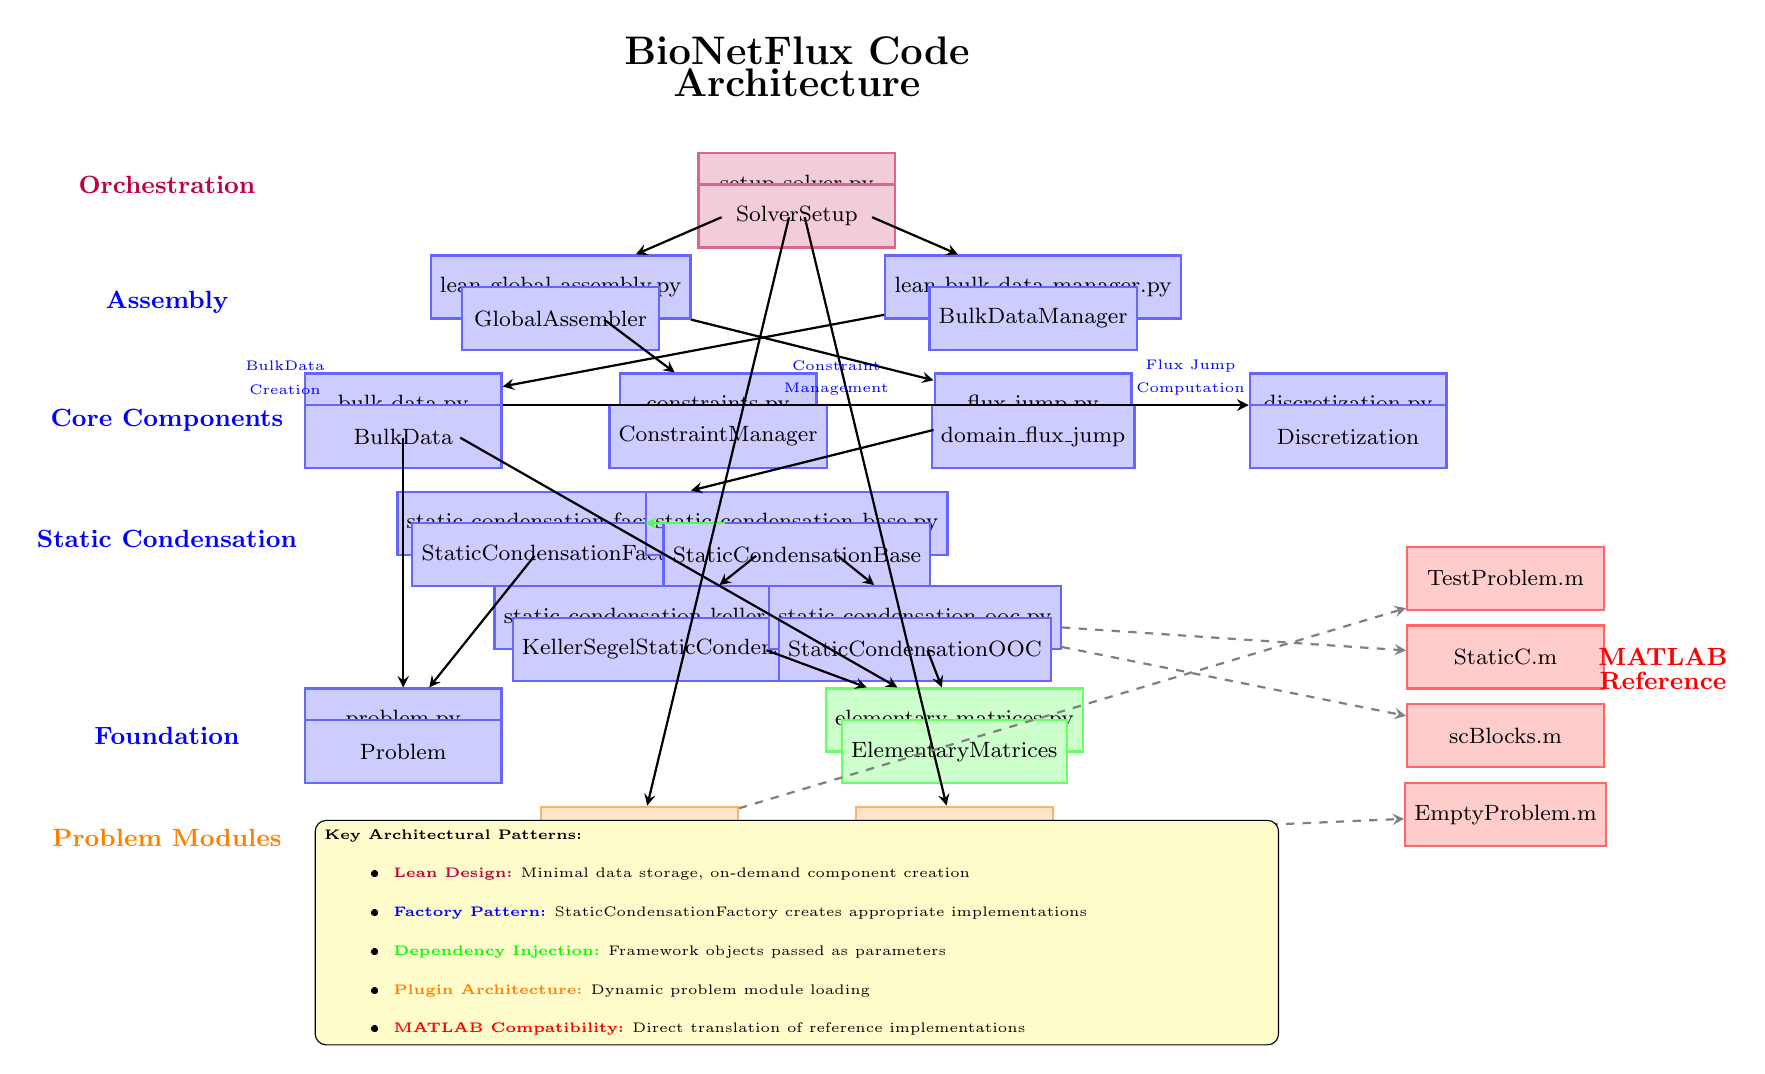
\begin{tikzpicture}[
    % Define styles
    core/.style={rectangle, draw=blue!60, fill=blue!20, thick, minimum width=2.5cm, minimum height=0.8cm, text centered, font=\footnotesize},
    utils/.style={rectangle, draw=green!60, fill=green!20, thick, minimum width=2.5cm, minimum height=0.8cm, text centered, font=\footnotesize},
    problems/.style={rectangle, draw=orange!60, fill=orange!20, thick, minimum width=2.5cm, minimum height=0.8cm, text centered, font=\footnotesize},
    setup/.style={rectangle, draw=purple!60, fill=purple!20, thick, minimum width=2.5cm, minimum height=0.8cm, text centered, font=\footnotesize},
    matlab/.style={rectangle, draw=red!60, fill=red!20, thick, minimum width=2.5cm, minimum height=0.8cm, text centered, font=\footnotesize},
    arrow/.style={->, thick, >=stealth},
    depends/.style={->, dashed, thick, >=stealth, color=gray},
    dataflow/.style={->, thick, >=stealth, color=blue!70},
    factory/.style={->, thick, >=stealth, color=green!70}
]

% Title - Split into two nodes
\node[font=\Large\bfseries] at (0, 10.2) {BioNetFlux Code};
\node[font=\Large\bfseries] at (0, 9.8) {Architecture};

% Layer 1: Setup and Orchestration (Top)
\node[setup] (setup_solver) at (0, 8.5) {setup\_solver.py};
\node[setup] (setup_solver_class) at (0, 8.1) {SolverSetup};

% Layer 2: Core Assembly (Upper Middle)
\node[core] (global_assembly) at (-3, 7.2) {lean\_global\_assembly.py};
\node[core] (global_assembly_class) at (-3, 6.8) {GlobalAssembler};
\node[core] (bulk_manager) at (3, 7.2) {lean\_bulk\_data\_manager.py};
\node[core] (bulk_manager_class) at (3, 6.8) {BulkDataManager};

% Layer 3: Core Components (Middle)
\node[core] (bulk_data) at (-5, 5.7) {bulk\_data.py};
\node[core] (bulk_data_class) at (-5, 5.3) {BulkData};
\node[core] (constraints) at (-1, 5.7) {constraints.py};
\node[core] (constraints_class) at (-1, 5.3) {ConstraintManager};
\node[core] (flux_jump) at (3, 5.7) {flux\_jump.py};
\node[core] (flux_jump_func) at (3, 5.3) {domain\_flux\_jump};
\node[core] (discretization) at (7, 5.7) {discretization.py};
\node[core] (discretization_class) at (7, 5.3) {Discretization};

% Layer 4: Static Condensation (Lower Middle)
\node[core] (sc_factory) at (-3, 4.2) {static\_condensation\_factory.py};
\node[core] (sc_factory_class) at (-3, 3.8) {StaticCondensationFactory};
\node[core] (sc_base) at (0, 4.2) {static\_condensation\_base.py};
\node[core] (sc_base_class) at (0, 3.8) {StaticCondensationBase};
\node[core] (sc_ks) at (-1.5, 3) {static\_condensation\_keller\_segel.py};
\node[core] (sc_ks_class) at (-1.5, 2.6) {KellerSegelStaticCondensation};
\node[core] (sc_ooc) at (1.5, 3) {static\_condensation\_ooc.py};
\node[core] (sc_ooc_class) at (1.5, 2.6) {StaticCondensationOOC};

% Layer 5: Foundation (Bottom)
\node[core] (problem) at (-5, 1.7) {problem.py};
\node[core] (problem_class) at (-5, 1.3) {Problem};
\node[utils] (elementary) at (2, 1.7) {elementary\_matrices.py};
\node[utils] (elementary_class) at (2, 1.3) {ElementaryMatrices};
\node[problems] (test_problem) at (-2, 0.2) {test\_problem2.py};
\node[problems] (double_arc) at (2, 0.2) {double\_arc.py};

% Layer 6: MATLAB Reference (Side)
\node[matlab] (matlab_test) at (9, 3.5) {TestProblem.m};
\node[matlab] (matlab_static) at (9, 2.5) {StaticC.m};
\node[matlab] (matlab_blocks) at (9, 1.5) {scBlocks.m};
\node[matlab] (matlab_empty) at (9, 0.5) {EmptyProblem.m};

% Main orchestration flow
\draw[arrow] (setup_solver) -- (global_assembly);
\draw[arrow] (setup_solver) -- (bulk_manager);

% Assembly dependencies
\draw[arrow] (global_assembly) -- (flux_jump);
\draw[arrow] (global_assembly) -- (constraints);
\draw[arrow] (bulk_manager) -- (bulk_data);

% Core component relationships
\draw[arrow] (flux_jump) -- (sc_factory);
\draw[arrow] (bulk_data) -- (elementary);
\draw[arrow] (bulk_data) -- (discretization);
\draw[arrow] (constraints) -- (discretization);

% Static condensation hierarchy
\draw[factory] (sc_factory) -- (sc_base);
\draw[arrow] (sc_base) -- (sc_ks);
\draw[arrow] (sc_base) -- (sc_ooc);
\draw[arrow] (sc_ks) -- (elementary);
\draw[arrow] (sc_ooc) -- (elementary);

% Problem dependencies
\draw[arrow] (bulk_data) -- (problem);
\draw[arrow] (sc_factory) -- (problem);
\draw[arrow] (setup_solver) -- (test_problem);
\draw[arrow] (setup_solver) -- (double_arc);

% MATLAB reference connections
\draw[depends] (sc_ooc) -- (matlab_static);
\draw[depends] (sc_ooc) -- (matlab_blocks);
\draw[depends] (test_problem) -- (matlab_test);
\draw[depends] (double_arc) -- (matlab_empty);

% Data flow annotations
\node[font=\tiny, color=blue] at (-6.5, 6.2) {BulkData};
\node[font=\tiny, color=blue] at (-6.5, 5.9) {Creation};
\node[font=\tiny, color=blue] at (0.5, 6.2) {Constraint};
\node[font=\tiny, color=blue] at (0.5, 5.9) {Management};
\node[font=\tiny, color=blue] at (5, 6.2) {Flux Jump};
\node[font=\tiny, color=blue] at (5, 5.9) {Computation};

% Layer labels
\node[font=\small\bfseries, color=purple] at (-8, 8.5) {Orchestration};
\node[font=\small\bfseries, color=blue] at (-8, 7) {Assembly};
\node[font=\small\bfseries, color=blue] at (-8, 5.5) {Core Components};
\node[font=\small\bfseries, color=blue] at (-8, 4) {Static Condensation};
\node[font=\small\bfseries, color=blue] at (-8, 1.5) {Foundation};
\node[font=\small\bfseries, color=orange] at (-8, 0.2) {Problem Modules};
\node[font=\small\bfseries, color=red] at (11, 2.5) {MATLAB};
\node[font=\small\bfseries, color=red] at (11, 2.2) {Reference};

% Key architectural patterns
\node[draw, rounded corners, fill=yellow!20, font=\tiny] at (0, -1) {
    \begin{minipage}{12cm}
    \textbf{Key Architectural Patterns:}
    \begin{itemize}
        \item \textcolor{purple}{\textbf{Lean Design:}} Minimal data storage, on-demand component creation
        \item \textcolor{blue}{\textbf{Factory Pattern:}} StaticCondensationFactory creates appropriate implementations
        \item \textcolor{green}{\textbf{Dependency Injection:}} Framework objects passed as parameters
        \item \textcolor{orange}{\textbf{Plugin Architecture:}} Dynamic problem module loading
        \item \textcolor{red}{\textbf{MATLAB Compatibility:}} Direct translation of reference implementations
    \end{itemize}
    \end{minipage}
};

\end{tikzpicture}
\caption[BioNetFlux Code Architecture]{
BioNetFlux code architecture showing the hierarchical structure and dependencies between modules. 
\textcolor{purple}{Purple boxes} represent orchestration layers, 
\textcolor{blue}{blue boxes} represent core computational components, 
\textcolor{green}{green boxes} represent utilities, 
\textcolor{orange}{orange boxes} represent problem-specific modules, and 
\textcolor{red}{red boxes} represent MATLAB reference implementations. 
Solid arrows indicate direct dependencies, dashed arrows indicate reference relationships, 
and colored arrows highlight specific architectural patterns (factory creation, data flow).
The lean design minimizes memory usage through on-demand component creation and parameter-based framework object passing.
}
\label{fig:bionetflux_architecture}
\end{figure}

% Supplementary detailed component diagram
\begin{figure}[htbp]
\centering
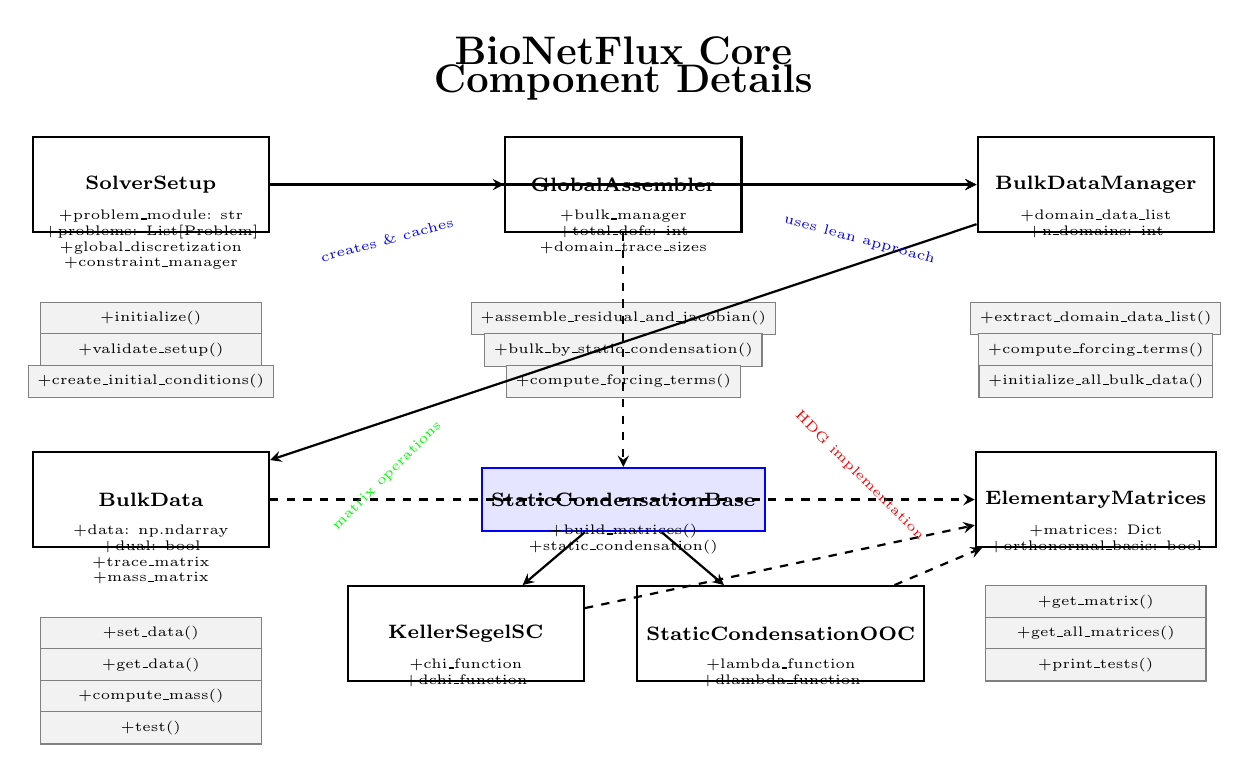
\begin{tikzpicture}[
    % Define styles - Fixed arrow tips
    class/.style={rectangle, draw=black, fill=white, thick, minimum width=3cm, minimum height=1.2cm, text centered, font=\scriptsize},
    method/.style={rectangle, draw=gray, fill=gray!10, minimum width=2.8cm, minimum height=0.4cm, text centered, font=\tiny},
    interface/.style={rectangle, draw=blue, fill=blue!10, thick, minimum width=3cm, minimum height=0.8cm, text centered, font=\scriptsize},
    composition/.style={->, thick, >=stealth},
    inheritance/.style={->, thick, >=stealth},
    usage/.style={->, dashed, thick, >=stealth}
]

% Title
\node[font=\Large\bfseries] at (0, 8.2) {BioNetFlux Core};
\node[font=\Large\bfseries] at (0, 7.8) {Component Details};

% SolverSetup detail
\node[class] (setup_detail) at (-6, 6.5) {
    \textbf{SolverSetup}
};
\node[font=\tiny] at (-6, 6.1) {+problem\_module: str};
\node[font=\tiny] at (-6, 5.9) {+problems: List[Problem]};
\node[font=\tiny] at (-6, 5.7) {+global\_discretization};
\node[font=\tiny] at (-6, 5.5) {+constraint\_manager};

\node[method] (setup_methods) at (-6, 4.8) {+initialize()};
\node[method] (setup_methods2) at (-6, 4.4) {+validate\_setup()};
\node[method] (setup_methods3) at (-6, 4.0) {+create\_initial\_conditions()};

% GlobalAssembler detail
\node[class] (assembler_detail) at (0, 6.5) {
    \textbf{GlobalAssembler}
};
\node[font=\tiny] at (0, 6.1) {+bulk\_manager};
\node[font=\tiny] at (0, 5.9) {+total\_dofs: int};
\node[font=\tiny] at (0, 5.7) {+domain\_trace\_sizes};

\node[method] (assembler_methods) at (0, 4.8) {+assemble\_residual\_and\_jacobian()};
\node[method] (assembler_methods2) at (0, 4.4) {+bulk\_by\_static\_condensation()};
\node[method] (assembler_methods3) at (0, 4.0) {+compute\_forcing\_terms()};

% BulkDataManager detail
\node[class] (manager_detail) at (6, 6.5) {
    \textbf{BulkDataManager}
};
\node[font=\tiny] at (6, 6.1) {+domain\_data\_list};
\node[font=\tiny] at (6, 5.9) {+n\_domains: int};

\node[method] (manager_methods) at (6, 4.8) {+extract\_domain\_data\_list()};
\node[method] (manager_methods2) at (6, 4.4) {+compute\_forcing\_terms()};
\node[method] (manager_methods3) at (6, 4.0) {+initialize\_all\_bulk\_data()};

% BulkData detail
\node[class] (bulk_detail) at (-6, 2.5) {
    \textbf{BulkData}
};
\node[font=\tiny] at (-6, 2.1) {+data: np.ndarray};
\node[font=\tiny] at (-6, 1.9) {+dual: bool};
\node[font=\tiny] at (-6, 1.7) {+trace\_matrix};
\node[font=\tiny] at (-6, 1.5) {+mass\_matrix};

\node[method] (bulk_methods) at (-6, 0.8) {+set\_data()};
\node[method] (bulk_methods2) at (-6, 0.4) {+get\_data()};
\node[method] (bulk_methods3) at (-6, 0.0) {+compute\_mass()};
\node[method] (bulk_methods4) at (-6, -0.4) {+test()};

% StaticCondensation hierarchy
\node[interface] (sc_interface) at (0, 2.5) {
    \textbf{StaticCondensationBase}
};
\node[font=\tiny] at (0, 2.1) {+build\_matrices()};
\node[font=\tiny] at (0, 1.9) {+static\_condensation()};

\node[class] (sc_ks_detail) at (-2, 0.8) {
    \textbf{KellerSegelSC}
};
\node[font=\tiny] at (-2, 0.4) {+chi\_function};
\node[font=\tiny] at (-2, 0.2) {+dchi\_function};

\node[class] (sc_ooc_detail) at (2, 0.8) {
    \textbf{StaticCondensationOOC}
};
\node[font=\tiny] at (2, 0.4) {+lambda\_function};
\node[font=\tiny] at (2, 0.2) {+dlambda\_function};

% ElementaryMatrices detail
\node[class] (elem_detail) at (6, 2.5) {
    \textbf{ElementaryMatrices}
};
\node[font=\tiny] at (6, 2.1) {+matrices: Dict};
\node[font=\tiny] at (6, 1.9) {+orthonormal\_basis: bool};

\node[method] (elem_methods) at (6, 1.2) {+get\_matrix()};
\node[method] (elem_methods2) at (6, 0.8) {+get\_all\_matrices()};
\node[method] (elem_methods3) at (6, 0.4) {+print\_tests()};

% Relationships - Using stealth arrow tips for all
\draw[composition] (setup_detail) -- (assembler_detail);
\draw[composition] (setup_detail) -- (manager_detail);
\draw[composition] (assembler_detail) -- (manager_detail);
\draw[composition] (manager_detail) -- (bulk_detail);
\draw[usage] (assembler_detail) -- (sc_interface);
\draw[inheritance] (sc_interface) -- (sc_ks_detail);
\draw[inheritance] (sc_interface) -- (sc_ooc_detail);
\draw[usage] (bulk_detail) -- (elem_detail);
\draw[usage] (sc_ks_detail) -- (elem_detail);
\draw[usage] (sc_ooc_detail) -- (elem_detail);

% Data flow indicators
\node[font=\tiny, color=blue, rotate=15] at (-3, 5.8) {creates \& caches};
\node[font=\tiny, color=blue, rotate=-15] at (3, 5.8) {uses lean approach};
\node[font=\tiny, color=green, rotate=45] at (-3, 2.8) {matrix operations};
\node[font=\tiny, color=red, rotate=-45] at (3, 2.8) {HDG implementation};

\end{tikzpicture}
\caption[BioNetFlux Component Details]{
Detailed view of key BioNetFlux components showing class structures, main attributes, and key methods. 
Solid arrows indicate composition and inheritance relationships, 
and dashed arrows represent usage dependencies. 
The diagram emphasizes the lean design pattern where components are created on-demand and cached for efficiency.
}
\label{fig:bionetflux_components}
\end{figure}

% Data flow diagram
\begin{figure}[htbp]
\centering
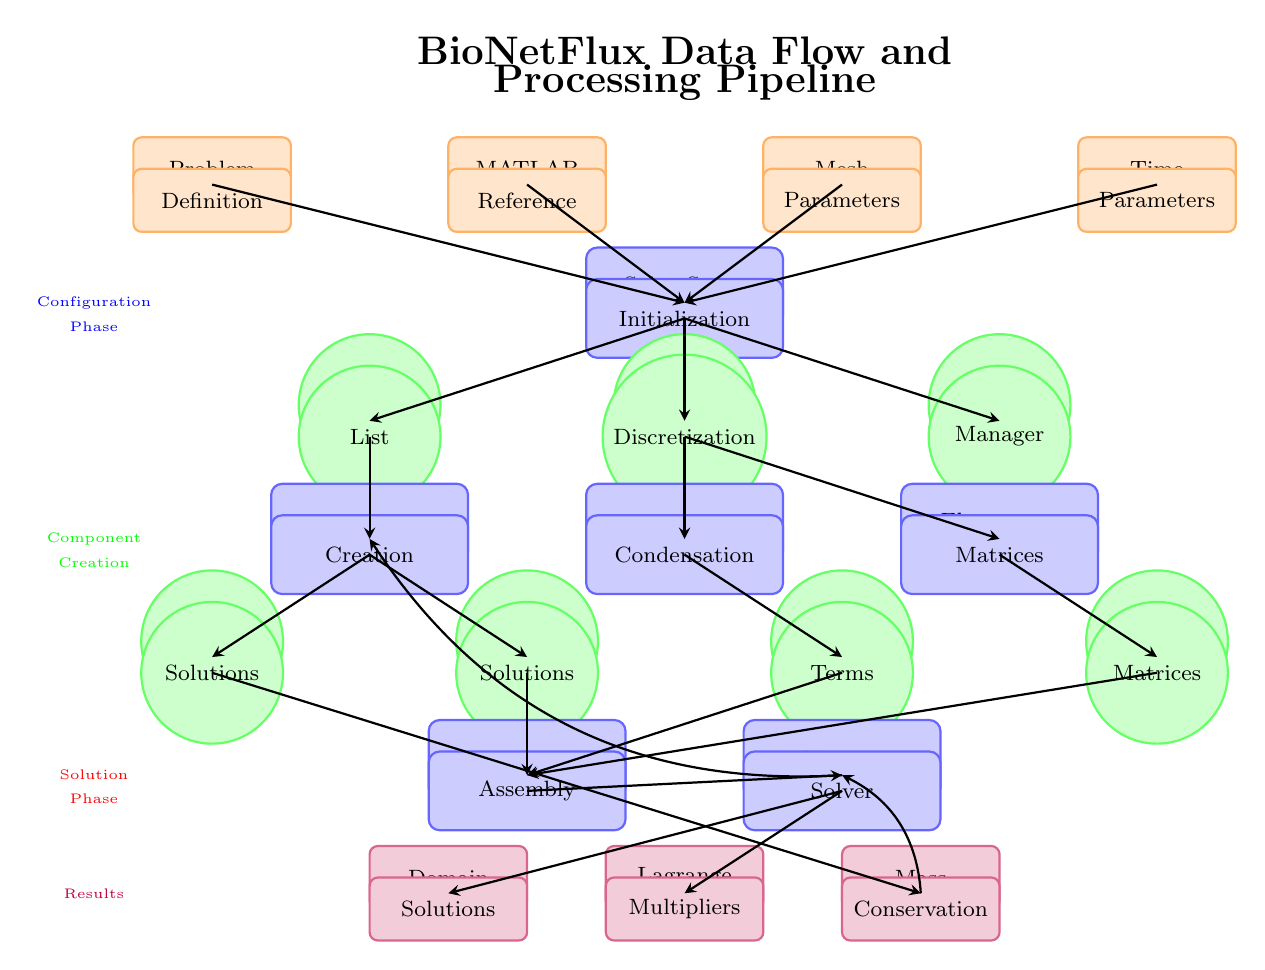
\begin{tikzpicture}[
    % Define styles - Fixed shapes using basic rectangles and circles
    process/.style={rectangle, rounded corners, draw=blue!60, fill=blue!20, thick, minimum width=2.5cm, minimum height=1cm, text centered, font=\footnotesize},
    data/.style={circle, draw=green!60, fill=green!20, thick, minimum width=1.8cm, text centered, font=\footnotesize},
    input/.style={rectangle, rounded corners=3pt, draw=orange!60, fill=orange!20, thick, minimum width=2cm, minimum height=0.8cm, text centered, font=\footnotesize},
    output/.style={rectangle, rounded corners=3pt, draw=purple!60, fill=purple!20, thick, minimum width=2cm, minimum height=0.8cm, text centered, font=\footnotesize},
    flow/.style={->, thick, >=stealth}
]

% Title
\node[font=\Large\bfseries] at (0, 9.2) {BioNetFlux Data Flow and};
\node[font=\Large\bfseries] at (0, 8.8) {Processing Pipeline};

% Input layer
\node[input] (problem_def_top) at (-6, 7.7) {Problem};
\node[input] (problem_def_bot) at (-6, 7.3) {Definition};
\node[input] (matlab_ref_top) at (-2, 7.7) {MATLAB};
\node[input] (matlab_ref_bot) at (-2, 7.3) {Reference};
\node[input] (mesh_params_top) at (2, 7.7) {Mesh};
\node[input] (mesh_params_bot) at (2, 7.3) {Parameters};
\node[input] (time_params_top) at (6, 7.7) {Time};
\node[input] (time_params_bot) at (6, 7.3) {Parameters};

% Processing layer 1: Setup
\node[process] (setup_process_top) at (0, 6.2) {SolverSetup};
\node[process] (setup_process_bot) at (0, 5.8) {Initialization};

% Data layer 1
\node[data] (problems_data_top) at (-4, 4.7) {Problems};
\node[data] (problems_data_bot) at (-4, 4.3) {List};
\node[data] (discretization_data_top) at (0, 4.7) {Global};
\node[data] (discretization_data_bot) at (0, 4.3) {Discretization};
\node[data] (constraints_data_top) at (4, 4.7) {Constraint};
\node[data] (constraints_data_bot) at (4, 4.3) {Manager};

% Processing layer 2: Component Creation
\node[process] (bulk_creation_top) at (-4, 3.2) {BulkData};
\node[process] (bulk_creation_bot) at (-4, 2.8) {Creation};
\node[process] (sc_creation_top) at (0, 3.2) {Static};
\node[process] (sc_creation_bot) at (0, 2.8) {Condensation};
\node[process] (matrix_creation_top) at (4, 3.2) {Elementary};
\node[process] (matrix_creation_bot) at (4, 2.8) {Matrices};

% Data layer 2
\node[data] (bulk_solutions_top) at (-6, 1.7) {Bulk};
\node[data] (bulk_solutions_bot) at (-6, 1.3) {Solutions};
\node[data] (trace_solutions_top) at (-2, 1.7) {Trace};
\node[data] (trace_solutions_bot) at (-2, 1.3) {Solutions};
\node[data] (forcing_terms_top) at (2, 1.7) {Forcing};
\node[data] (forcing_terms_bot) at (2, 1.3) {Terms};
\node[data] (matrices_top) at (6, 1.7) {System};
\node[data] (matrices_bot) at (6, 1.3) {Matrices};

% Processing layer 3: Assembly and Solving
\node[process] (assembly_process_top) at (-2, 0.2) {Global};
\node[process] (assembly_process_bot) at (-2, -0.2) {Assembly};
\node[process] (newton_process_top) at (2, 0.2) {Newton};
\node[process] (newton_process_bot) at (2, -0.2) {Solver};

% Output layer
\node[output] (solution_output_top) at (-3, -1.3) {Domain};
\node[output] (solution_output_bot) at (-3, -1.7) {Solutions};
\node[output] (multiplier_output_top) at (0, -1.3) {Lagrange};
\node[output] (multiplier_output_bot) at (0, -1.7) {Multipliers};
\node[output] (conservation_output_top) at (3, -1.3) {Mass};
\node[output] (conservation_output_bot) at (3, -1.7) {Conservation};

% Flow connections (connecting to center points)
\draw[flow] (-6, 7.5) -- (0, 6);
\draw[flow] (-2, 7.5) -- (0, 6);
\draw[flow] (2, 7.5) -- (0, 6);
\draw[flow] (6, 7.5) -- (0, 6);

\draw[flow] (0, 5.8) -- (-4, 4.5);
\draw[flow] (0, 5.8) -- (0, 4.5);
\draw[flow] (0, 5.8) -- (4, 4.5);

\draw[flow] (-4, 4.3) -- (-4, 3);
\draw[flow] (0, 4.3) -- (0, 3);
\draw[flow] (0, 4.3) -- (4, 3);

\draw[flow] (-4, 2.8) -- (-6, 1.5);
\draw[flow] (-4, 2.8) -- (-2, 1.5);
\draw[flow] (0, 2.8) -- (2, 1.5);
\draw[flow] (4, 2.8) -- (6, 1.5);

\draw[flow] (-2, 1.3) -- (-2, 0);
\draw[flow] (2, 1.3) -- (-2, 0);
\draw[flow] (6, 1.3) -- (-2, 0);
\draw[flow] (-2, -0.2) -- (2, 0);

\draw[flow] (2, -0.2) -- (-3, -1.5);
\draw[flow] (2, -0.2) -- (0, -1.5);
\draw[flow] (-6, 1.3) -- (3, -1.5);

% Feedback loops
\draw[flow, bend left=30] (2, 0) to (-4, 3);
\draw[flow, bend right=30] (3, -1.5) to (2, 0);

% Annotations
\node[font=\tiny, color=blue] at (-7.5, 6) {Configuration};
\node[font=\tiny, color=blue] at (-7.5, 5.7) {Phase};
\node[font=\tiny, color=green] at (-7.5, 3) {Component};
\node[font=\tiny, color=green] at (-7.5, 2.7) {Creation};
\node[font=\tiny, color=red] at (-7.5, 0) {Solution};
\node[font=\tiny, color=red] at (-7.5, -0.3) {Phase};
\node[font=\tiny, color=purple] at (-7.5, -1.5) {Results};

\end{tikzpicture}
\caption[BioNetFlux Data Flow]{
BioNetFlux data flow and processing pipeline showing the transformation from input parameters through component creation to final solutions. 
Orange rectangles represent input data, blue rounded rectangles represent processing steps, 
green circles represent intermediate data structures, and purple rectangles represent outputs. 
The diagram illustrates the lean approach where components are created on-demand and data flows efficiently through the processing pipeline.
Feedback loops show the iterative nature of the Newton solver and mass conservation monitoring.
}
\label{fig:bionetflux_dataflow}
\end{figure}


\begin{figure}[htbp]
\centering
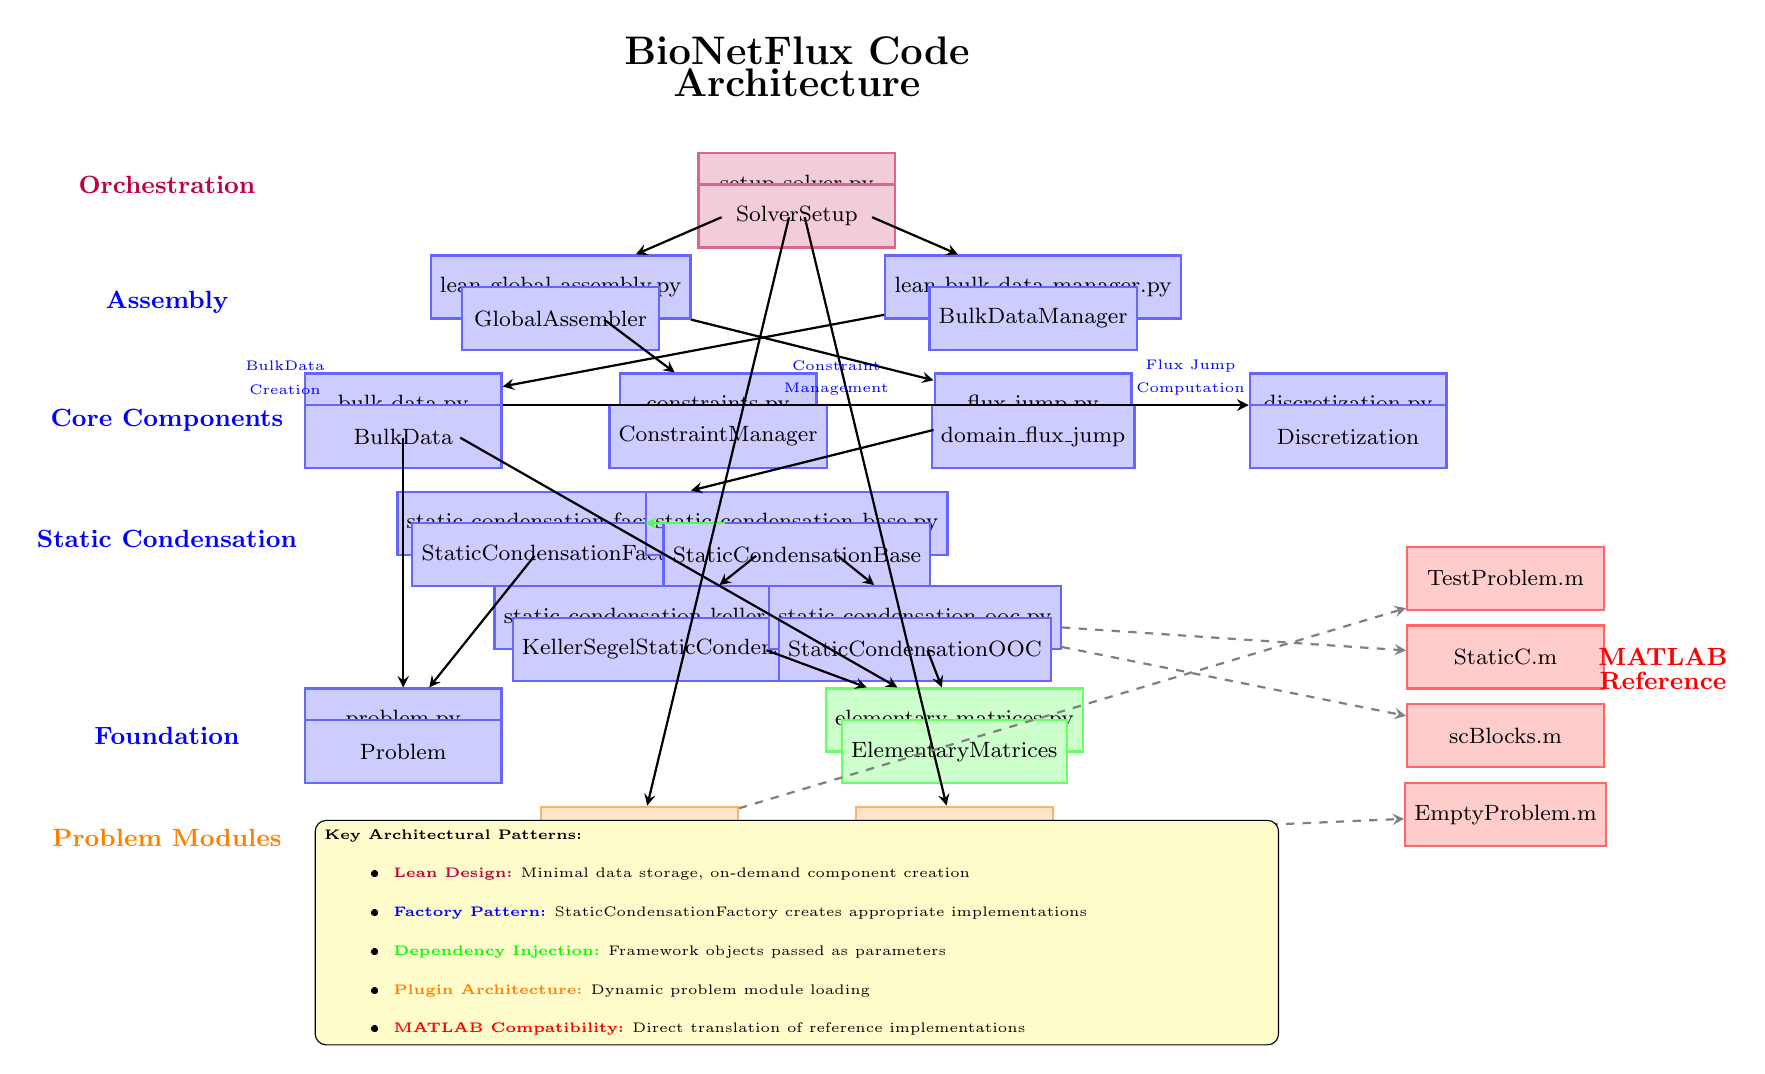
\begin{tikzpicture}[
    % Define styles
    core/.style={rectangle, draw=blue!60, fill=blue!20, thick, minimum width=2.5cm, minimum height=0.8cm, text centered, font=\footnotesize},
    utils/.style={rectangle, draw=green!60, fill=green!20, thick, minimum width=2.5cm, minimum height=0.8cm, text centered, font=\footnotesize},
    problems/.style={rectangle, draw=orange!60, fill=orange!20, thick, minimum width=2.5cm, minimum height=0.8cm, text centered, font=\footnotesize},
    setup/.style={rectangle, draw=purple!60, fill=purple!20, thick, minimum width=2.5cm, minimum height=0.8cm, text centered, font=\footnotesize},
    matlab/.style={rectangle, draw=red!60, fill=red!20, thick, minimum width=2.5cm, minimum height=0.8cm, text centered, font=\footnotesize},
    arrow/.style={->, thick, >=stealth},
    depends/.style={->, dashed, thick, >=stealth, color=gray},
    dataflow/.style={->, thick, >=stealth, color=blue!70},
    factory/.style={->, thick, >=stealth, color=green!70}
]

% Title - Split into two nodes
\node[font=\Large\bfseries] at (0, 10.2) {BioNetFlux Code};
\node[font=\Large\bfseries] at (0, 9.8) {Architecture};

% Layer 1: Setup and Orchestration (Top)
\node[setup] (setup_solver) at (0, 8.5) {setup\_solver.py};
\node[setup] (setup_solver_class) at (0, 8.1) {SolverSetup};

% Layer 2: Core Assembly (Upper Middle)
\node[core] (global_assembly) at (-3, 7.2) {lean\_global\_assembly.py};
\node[core] (global_assembly_class) at (-3, 6.8) {GlobalAssembler};
\node[core] (bulk_manager) at (3, 7.2) {lean\_bulk\_data\_manager.py};
\node[core] (bulk_manager_class) at (3, 6.8) {BulkDataManager};

% Layer 3: Core Components (Middle)
\node[core] (bulk_data) at (-5, 5.7) {bulk\_data.py};
\node[core] (bulk_data_class) at (-5, 5.3) {BulkData};
\node[core] (constraints) at (-1, 5.7) {constraints.py};
\node[core] (constraints_class) at (-1, 5.3) {ConstraintManager};
\node[core] (flux_jump) at (3, 5.7) {flux\_jump.py};
\node[core] (flux_jump_func) at (3, 5.3) {domain\_flux\_jump};
\node[core] (discretization) at (7, 5.7) {discretization.py};
\node[core] (discretization_class) at (7, 5.3) {Discretization};

% Layer 4: Static Condensation (Lower Middle)
\node[core] (sc_factory) at (-3, 4.2) {static\_condensation\_factory.py};
\node[core] (sc_factory_class) at (-3, 3.8) {StaticCondensationFactory};
\node[core] (sc_base) at (0, 4.2) {static\_condensation\_base.py};
\node[core] (sc_base_class) at (0, 3.8) {StaticCondensationBase};
\node[core] (sc_ks) at (-1.5, 3) {static\_condensation\_keller\_segel.py};
\node[core] (sc_ks_class) at (-1.5, 2.6) {KellerSegelStaticCondensation};
\node[core] (sc_ooc) at (1.5, 3) {static\_condensation\_ooc.py};
\node[core] (sc_ooc_class) at (1.5, 2.6) {StaticCondensationOOC};

% Layer 5: Foundation (Bottom)
\node[core] (problem) at (-5, 1.7) {problem.py};
\node[core] (problem_class) at (-5, 1.3) {Problem};
\node[utils] (elementary) at (2, 1.7) {elementary\_matrices.py};
\node[utils] (elementary_class) at (2, 1.3) {ElementaryMatrices};
\node[problems] (test_problem) at (-2, 0.2) {test\_problem2.py};
\node[problems] (double_arc) at (2, 0.2) {double\_arc.py};

% Layer 6: MATLAB Reference (Side)
\node[matlab] (matlab_test) at (9, 3.5) {TestProblem.m};
\node[matlab] (matlab_static) at (9, 2.5) {StaticC.m};
\node[matlab] (matlab_blocks) at (9, 1.5) {scBlocks.m};
\node[matlab] (matlab_empty) at (9, 0.5) {EmptyProblem.m};

% Main orchestration flow
\draw[arrow] (setup_solver) -- (global_assembly);
\draw[arrow] (setup_solver) -- (bulk_manager);

% Assembly dependencies
\draw[arrow] (global_assembly) -- (flux_jump);
\draw[arrow] (global_assembly) -- (constraints);
\draw[arrow] (bulk_manager) -- (bulk_data);

% Core component relationships
\draw[arrow] (flux_jump) -- (sc_factory);
\draw[arrow] (bulk_data) -- (elementary);
\draw[arrow] (bulk_data) -- (discretization);
\draw[arrow] (constraints) -- (discretization);

% Static condensation hierarchy
\draw[factory] (sc_factory) -- (sc_base);
\draw[arrow] (sc_base) -- (sc_ks);
\draw[arrow] (sc_base) -- (sc_ooc);
\draw[arrow] (sc_ks) -- (elementary);
\draw[arrow] (sc_ooc) -- (elementary);

% Problem dependencies
\draw[arrow] (bulk_data) -- (problem);
\draw[arrow] (sc_factory) -- (problem);
\draw[arrow] (setup_solver) -- (test_problem);
\draw[arrow] (setup_solver) -- (double_arc);

% MATLAB reference connections
\draw[depends] (sc_ooc) -- (matlab_static);
\draw[depends] (sc_ooc) -- (matlab_blocks);
\draw[depends] (test_problem) -- (matlab_test);
\draw[depends] (double_arc) -- (matlab_empty);

% Data flow annotations
\node[font=\tiny, color=blue] at (-6.5, 6.2) {BulkData};
\node[font=\tiny, color=blue] at (-6.5, 5.9) {Creation};
\node[font=\tiny, color=blue] at (0.5, 6.2) {Constraint};
\node[font=\tiny, color=blue] at (0.5, 5.9) {Management};
\node[font=\tiny, color=blue] at (5, 6.2) {Flux Jump};
\node[font=\tiny, color=blue] at (5, 5.9) {Computation};

% Layer labels
\node[font=\small\bfseries, color=purple] at (-8, 8.5) {Orchestration};
\node[font=\small\bfseries, color=blue] at (-8, 7) {Assembly};
\node[font=\small\bfseries, color=blue] at (-8, 5.5) {Core Components};
\node[font=\small\bfseries, color=blue] at (-8, 4) {Static Condensation};
\node[font=\small\bfseries, color=blue] at (-8, 1.5) {Foundation};
\node[font=\small\bfseries, color=orange] at (-8, 0.2) {Problem Modules};
\node[font=\small\bfseries, color=red] at (11, 2.5) {MATLAB};
\node[font=\small\bfseries, color=red] at (11, 2.2) {Reference};

% Key architectural patterns
\node[draw, rounded corners, fill=yellow!20, font=\tiny] at (0, -1) {
    \begin{minipage}{12cm}
    \textbf{Key Architectural Patterns:}
    \begin{itemize}
        \item \textcolor{purple}{\textbf{Lean Design:}} Minimal data storage, on-demand component creation
        \item \textcolor{blue}{\textbf{Factory Pattern:}} StaticCondensationFactory creates appropriate implementations
        \item \textcolor{green}{\textbf{Dependency Injection:}} Framework objects passed as parameters
        \item \textcolor{orange}{\textbf{Plugin Architecture:}} Dynamic problem module loading
        \item \textcolor{red}{\textbf{MATLAB Compatibility:}} Direct translation of reference implementations
    \end{itemize}
    \end{minipage}
};

\end{tikzpicture}
\caption[BioNetFlux Code Architecture]{
BioNetFlux code architecture showing the hierarchical structure and dependencies between modules. 
\textcolor{purple}{Purple boxes} represent orchestration layers, 
\textcolor{blue}{blue boxes} represent core computational components, 
\textcolor{green}{green boxes} represent utilities, 
\textcolor{orange}{orange boxes} represent problem-specific modules, and 
\textcolor{red}{red boxes} represent MATLAB reference implementations. 
Solid arrows indicate direct dependencies, dashed arrows indicate reference relationships, 
and colored arrows highlight specific architectural patterns (factory creation, data flow).
The lean design minimizes memory usage through on-demand component creation and parameter-based framework object passing.
}
\label{fig:bionetflux_architecture}
\end{figure}

% Supplementary detailed component diagram
\begin{figure}[htbp]
\centering
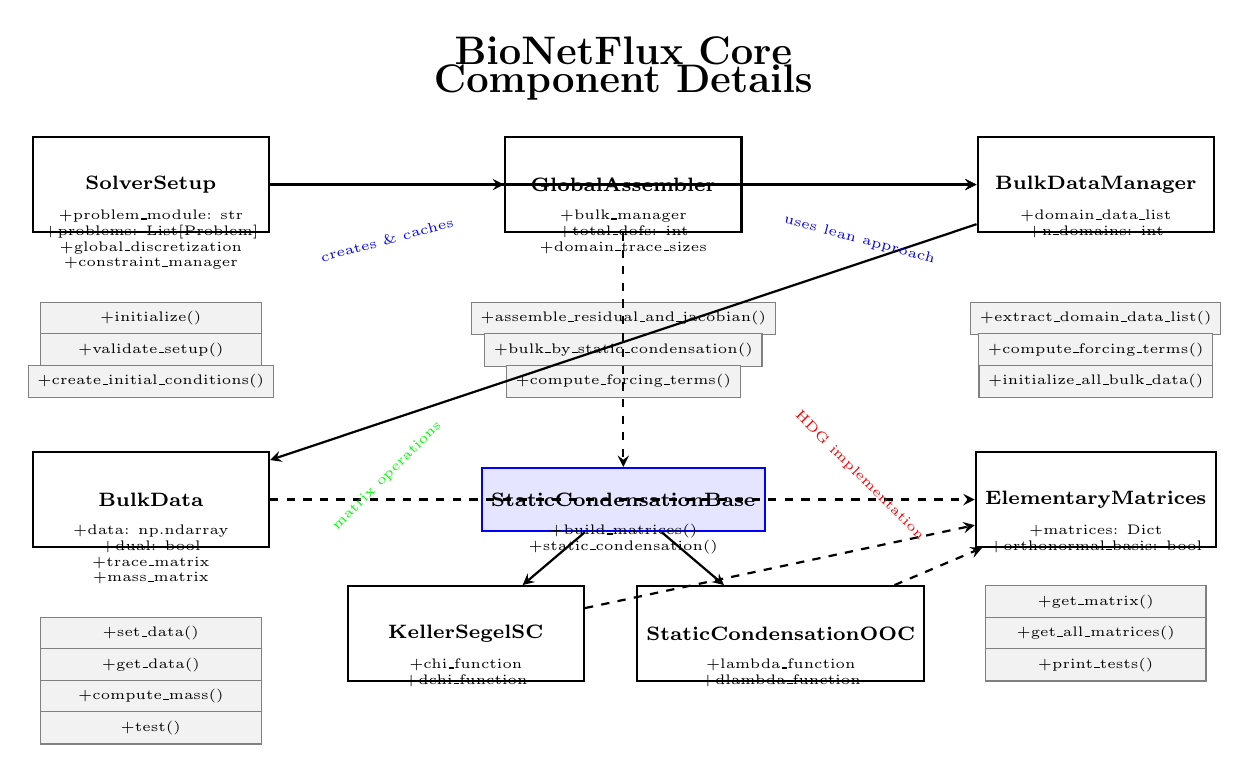
\begin{tikzpicture}[
    % Define styles - Fixed arrow tips
    class/.style={rectangle, draw=black, fill=white, thick, minimum width=3cm, minimum height=1.2cm, text centered, font=\scriptsize},
    method/.style={rectangle, draw=gray, fill=gray!10, minimum width=2.8cm, minimum height=0.4cm, text centered, font=\tiny},
    interface/.style={rectangle, draw=blue, fill=blue!10, thick, minimum width=3cm, minimum height=0.8cm, text centered, font=\scriptsize},
    composition/.style={->, thick, >=stealth},
    inheritance/.style={->, thick, >=stealth},
    usage/.style={->, dashed, thick, >=stealth}
]

% Title
\node[font=\Large\bfseries] at (0, 8.2) {BioNetFlux Core};
\node[font=\Large\bfseries] at (0, 7.8) {Component Details};

% SolverSetup detail
\node[class] (setup_detail) at (-6, 6.5) {
    \textbf{SolverSetup}
};
\node[font=\tiny] at (-6, 6.1) {+problem\_module: str};
\node[font=\tiny] at (-6, 5.9) {+problems: List[Problem]};
\node[font=\tiny] at (-6, 5.7) {+global\_discretization};
\node[font=\tiny] at (-6, 5.5) {+constraint\_manager};

\node[method] (setup_methods) at (-6, 4.8) {+initialize()};
\node[method] (setup_methods2) at (-6, 4.4) {+validate\_setup()};
\node[method] (setup_methods3) at (-6, 4.0) {+create\_initial\_conditions()};

% GlobalAssembler detail
\node[class] (assembler_detail) at (0, 6.5) {
    \textbf{GlobalAssembler}
};
\node[font=\tiny] at (0, 6.1) {+bulk\_manager};
\node[font=\tiny] at (0, 5.9) {+total\_dofs: int};
\node[font=\tiny] at (0, 5.7) {+domain\_trace\_sizes};

\node[method] (assembler_methods) at (0, 4.8) {+assemble\_residual\_and\_jacobian()};
\node[method] (assembler_methods2) at (0, 4.4) {+bulk\_by\_static\_condensation()};
\node[method] (assembler_methods3) at (0, 4.0) {+compute\_forcing\_terms()};

% BulkDataManager detail
\node[class] (manager_detail) at (6, 6.5) {
    \textbf{BulkDataManager}
};
\node[font=\tiny] at (6, 6.1) {+domain\_data\_list};
\node[font=\tiny] at (6, 5.9) {+n\_domains: int};

\node[method] (manager_methods) at (6, 4.8) {+extract\_domain\_data\_list()};
\node[method] (manager_methods2) at (6, 4.4) {+compute\_forcing\_terms()};
\node[method] (manager_methods3) at (6, 4.0) {+initialize\_all\_bulk\_data()};

% BulkData detail
\node[class] (bulk_detail) at (-6, 2.5) {
    \textbf{BulkData}
};
\node[font=\tiny] at (-6, 2.1) {+data: np.ndarray};
\node[font=\tiny] at (-6, 1.9) {+dual: bool};
\node[font=\tiny] at (-6, 1.7) {+trace\_matrix};
\node[font=\tiny] at (-6, 1.5) {+mass\_matrix};

\node[method] (bulk_methods) at (-6, 0.8) {+set\_data()};
\node[method] (bulk_methods2) at (-6, 0.4) {+get\_data()};
\node[method] (bulk_methods3) at (-6, 0.0) {+compute\_mass()};
\node[method] (bulk_methods4) at (-6, -0.4) {+test()};

% StaticCondensation hierarchy
\node[interface] (sc_interface) at (0, 2.5) {
    \textbf{StaticCondensationBase}
};
\node[font=\tiny] at (0, 2.1) {+build\_matrices()};
\node[font=\tiny] at (0, 1.9) {+static\_condensation()};

\node[class] (sc_ks_detail) at (-2, 0.8) {
    \textbf{KellerSegelSC}
};
\node[font=\tiny] at (-2, 0.4) {+chi\_function};
\node[font=\tiny] at (-2, 0.2) {+dchi\_function};

\node[class] (sc_ooc_detail) at (2, 0.8) {
    \textbf{StaticCondensationOOC}
};
\node[font=\tiny] at (2, 0.4) {+lambda\_function};
\node[font=\tiny] at (2, 0.2) {+dlambda\_function};

% ElementaryMatrices detail
\node[class] (elem_detail) at (6, 2.5) {
    \textbf{ElementaryMatrices}
};
\node[font=\tiny] at (6, 2.1) {+matrices: Dict};
\node[font=\tiny] at (6, 1.9) {+orthonormal\_basis: bool};

\node[method] (elem_methods) at (6, 1.2) {+get\_matrix()};
\node[method] (elem_methods2) at (6, 0.8) {+get\_all\_matrices()};
\node[method] (elem_methods3) at (6, 0.4) {+print\_tests()};

% Relationships - Using stealth arrow tips for all
\draw[composition] (setup_detail) -- (assembler_detail);
\draw[composition] (setup_detail) -- (manager_detail);
\draw[composition] (assembler_detail) -- (manager_detail);
\draw[composition] (manager_detail) -- (bulk_detail);
\draw[usage] (assembler_detail) -- (sc_interface);
\draw[inheritance] (sc_interface) -- (sc_ks_detail);
\draw[inheritance] (sc_interface) -- (sc_ooc_detail);
\draw[usage] (bulk_detail) -- (elem_detail);
\draw[usage] (sc_ks_detail) -- (elem_detail);
\draw[usage] (sc_ooc_detail) -- (elem_detail);

% Data flow indicators
\node[font=\tiny, color=blue, rotate=15] at (-3, 5.8) {creates \& caches};
\node[font=\tiny, color=blue, rotate=-15] at (3, 5.8) {uses lean approach};
\node[font=\tiny, color=green, rotate=45] at (-3, 2.8) {matrix operations};
\node[font=\tiny, color=red, rotate=-45] at (3, 2.8) {HDG implementation};

\end{tikzpicture}
\caption[BioNetFlux Component Details]{
Detailed view of key BioNetFlux components showing class structures, main attributes, and key methods. 
Solid arrows indicate composition and inheritance relationships, 
and dashed arrows represent usage dependencies. 
The diagram emphasizes the lean design pattern where components are created on-demand and cached for efficiency.
}
\label{fig:bionetflux_components}
\end{figure}

% Data flow diagram
\begin{figure}[htbp]
\centering
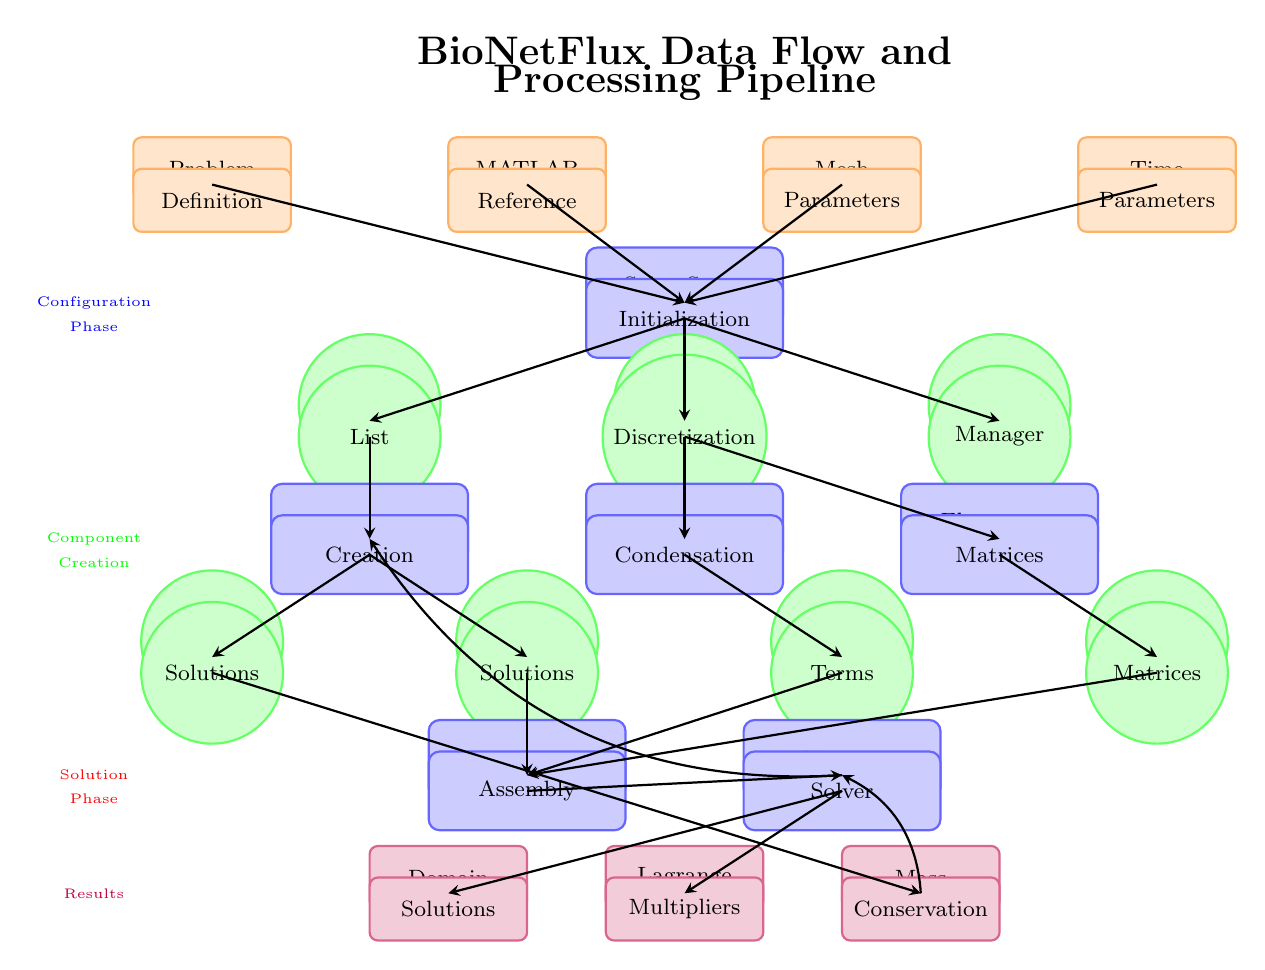
\begin{tikzpicture}[
    % Define styles - Fixed shapes using basic rectangles and circles
    process/.style={rectangle, rounded corners, draw=blue!60, fill=blue!20, thick, minimum width=2.5cm, minimum height=1cm, text centered, font=\footnotesize},
    data/.style={circle, draw=green!60, fill=green!20, thick, minimum width=1.8cm, text centered, font=\footnotesize},
    input/.style={rectangle, rounded corners=3pt, draw=orange!60, fill=orange!20, thick, minimum width=2cm, minimum height=0.8cm, text centered, font=\footnotesize},
    output/.style={rectangle, rounded corners=3pt, draw=purple!60, fill=purple!20, thick, minimum width=2cm, minimum height=0.8cm, text centered, font=\footnotesize},
    flow/.style={->, thick, >=stealth}
]

% Title
\node[font=\Large\bfseries] at (0, 9.2) {BioNetFlux Data Flow and};
\node[font=\Large\bfseries] at (0, 8.8) {Processing Pipeline};

% Input layer
\node[input] (problem_def_top) at (-6, 7.7) {Problem};
\node[input] (problem_def_bot) at (-6, 7.3) {Definition};
\node[input] (matlab_ref_top) at (-2, 7.7) {MATLAB};
\node[input] (matlab_ref_bot) at (-2, 7.3) {Reference};
\node[input] (mesh_params_top) at (2, 7.7) {Mesh};
\node[input] (mesh_params_bot) at (2, 7.3) {Parameters};
\node[input] (time_params_top) at (6, 7.7) {Time};
\node[input] (time_params_bot) at (6, 7.3) {Parameters};

% Processing layer 1: Setup
\node[process] (setup_process_top) at (0, 6.2) {SolverSetup};
\node[process] (setup_process_bot) at (0, 5.8) {Initialization};

% Data layer 1
\node[data] (problems_data_top) at (-4, 4.7) {Problems};
\node[data] (problems_data_bot) at (-4, 4.3) {List};
\node[data] (discretization_data_top) at (0, 4.7) {Global};
\node[data] (discretization_data_bot) at (0, 4.3) {Discretization};
\node[data] (constraints_data_top) at (4, 4.7) {Constraint};
\node[data] (constraints_data_bot) at (4, 4.3) {Manager};

% Processing layer 2: Component Creation
\node[process] (bulk_creation_top) at (-4, 3.2) {BulkData};
\node[process] (bulk_creation_bot) at (-4, 2.8) {Creation};
\node[process] (sc_creation_top) at (0, 3.2) {Static};
\node[process] (sc_creation_bot) at (0, 2.8) {Condensation};
\node[process] (matrix_creation_top) at (4, 3.2) {Elementary};
\node[process] (matrix_creation_bot) at (4, 2.8) {Matrices};

% Data layer 2
\node[data] (bulk_solutions_top) at (-6, 1.7) {Bulk};
\node[data] (bulk_solutions_bot) at (-6, 1.3) {Solutions};
\node[data] (trace_solutions_top) at (-2, 1.7) {Trace};
\node[data] (trace_solutions_bot) at (-2, 1.3) {Solutions};
\node[data] (forcing_terms_top) at (2, 1.7) {Forcing};
\node[data] (forcing_terms_bot) at (2, 1.3) {Terms};
\node[data] (matrices_top) at (6, 1.7) {System};
\node[data] (matrices_bot) at (6, 1.3) {Matrices};

% Processing layer 3: Assembly and Solving
\node[process] (assembly_process_top) at (-2, 0.2) {Global};
\node[process] (assembly_process_bot) at (-2, -0.2) {Assembly};
\node[process] (newton_process_top) at (2, 0.2) {Newton};
\node[process] (newton_process_bot) at (2, -0.2) {Solver};

% Output layer
\node[output] (solution_output_top) at (-3, -1.3) {Domain};
\node[output] (solution_output_bot) at (-3, -1.7) {Solutions};
\node[output] (multiplier_output_top) at (0, -1.3) {Lagrange};
\node[output] (multiplier_output_bot) at (0, -1.7) {Multipliers};
\node[output] (conservation_output_top) at (3, -1.3) {Mass};
\node[output] (conservation_output_bot) at (3, -1.7) {Conservation};

% Flow connections (connecting to center points)
\draw[flow] (-6, 7.5) -- (0, 6);
\draw[flow] (-2, 7.5) -- (0, 6);
\draw[flow] (2, 7.5) -- (0, 6);
\draw[flow] (6, 7.5) -- (0, 6);

\draw[flow] (0, 5.8) -- (-4, 4.5);
\draw[flow] (0, 5.8) -- (0, 4.5);
\draw[flow] (0, 5.8) -- (4, 4.5);

\draw[flow] (-4, 4.3) -- (-4, 3);
\draw[flow] (0, 4.3) -- (0, 3);
\draw[flow] (0, 4.3) -- (4, 3);

\draw[flow] (-4, 2.8) -- (-6, 1.5);
\draw[flow] (-4, 2.8) -- (-2, 1.5);
\draw[flow] (0, 2.8) -- (2, 1.5);
\draw[flow] (4, 2.8) -- (6, 1.5);

\draw[flow] (-2, 1.3) -- (-2, 0);
\draw[flow] (2, 1.3) -- (-2, 0);
\draw[flow] (6, 1.3) -- (-2, 0);
\draw[flow] (-2, -0.2) -- (2, 0);

\draw[flow] (2, -0.2) -- (-3, -1.5);
\draw[flow] (2, -0.2) -- (0, -1.5);
\draw[flow] (-6, 1.3) -- (3, -1.5);

% Feedback loops
\draw[flow, bend left=30] (2, 0) to (-4, 3);
\draw[flow, bend right=30] (3, -1.5) to (2, 0);

% Annotations
\node[font=\tiny, color=blue] at (-7.5, 6) {Configuration};
\node[font=\tiny, color=blue] at (-7.5, 5.7) {Phase};
\node[font=\tiny, color=green] at (-7.5, 3) {Component};
\node[font=\tiny, color=green] at (-7.5, 2.7) {Creation};
\node[font=\tiny, color=red] at (-7.5, 0) {Solution};
\node[font=\tiny, color=red] at (-7.5, -0.3) {Phase};
\node[font=\tiny, color=purple] at (-7.5, -1.5) {Results};

\end{tikzpicture}
\caption[BioNetFlux Data Flow]{
BioNetFlux data flow and processing pipeline showing the transformation from input parameters through component creation to final solutions. 
Orange rectangles represent input data, blue rounded rectangles represent processing steps, 
green circles represent intermediate data structures, and purple rectangles represent outputs. 
The diagram illustrates the lean approach where components are created on-demand and data flows efficiently through the processing pipeline.
Feedback loops show the iterative nature of the Newton solver and mass conservation monitoring.
}
\label{fig:bionetflux_dataflow}
\end{figure}


\begin{figure}[htbp]
\centering
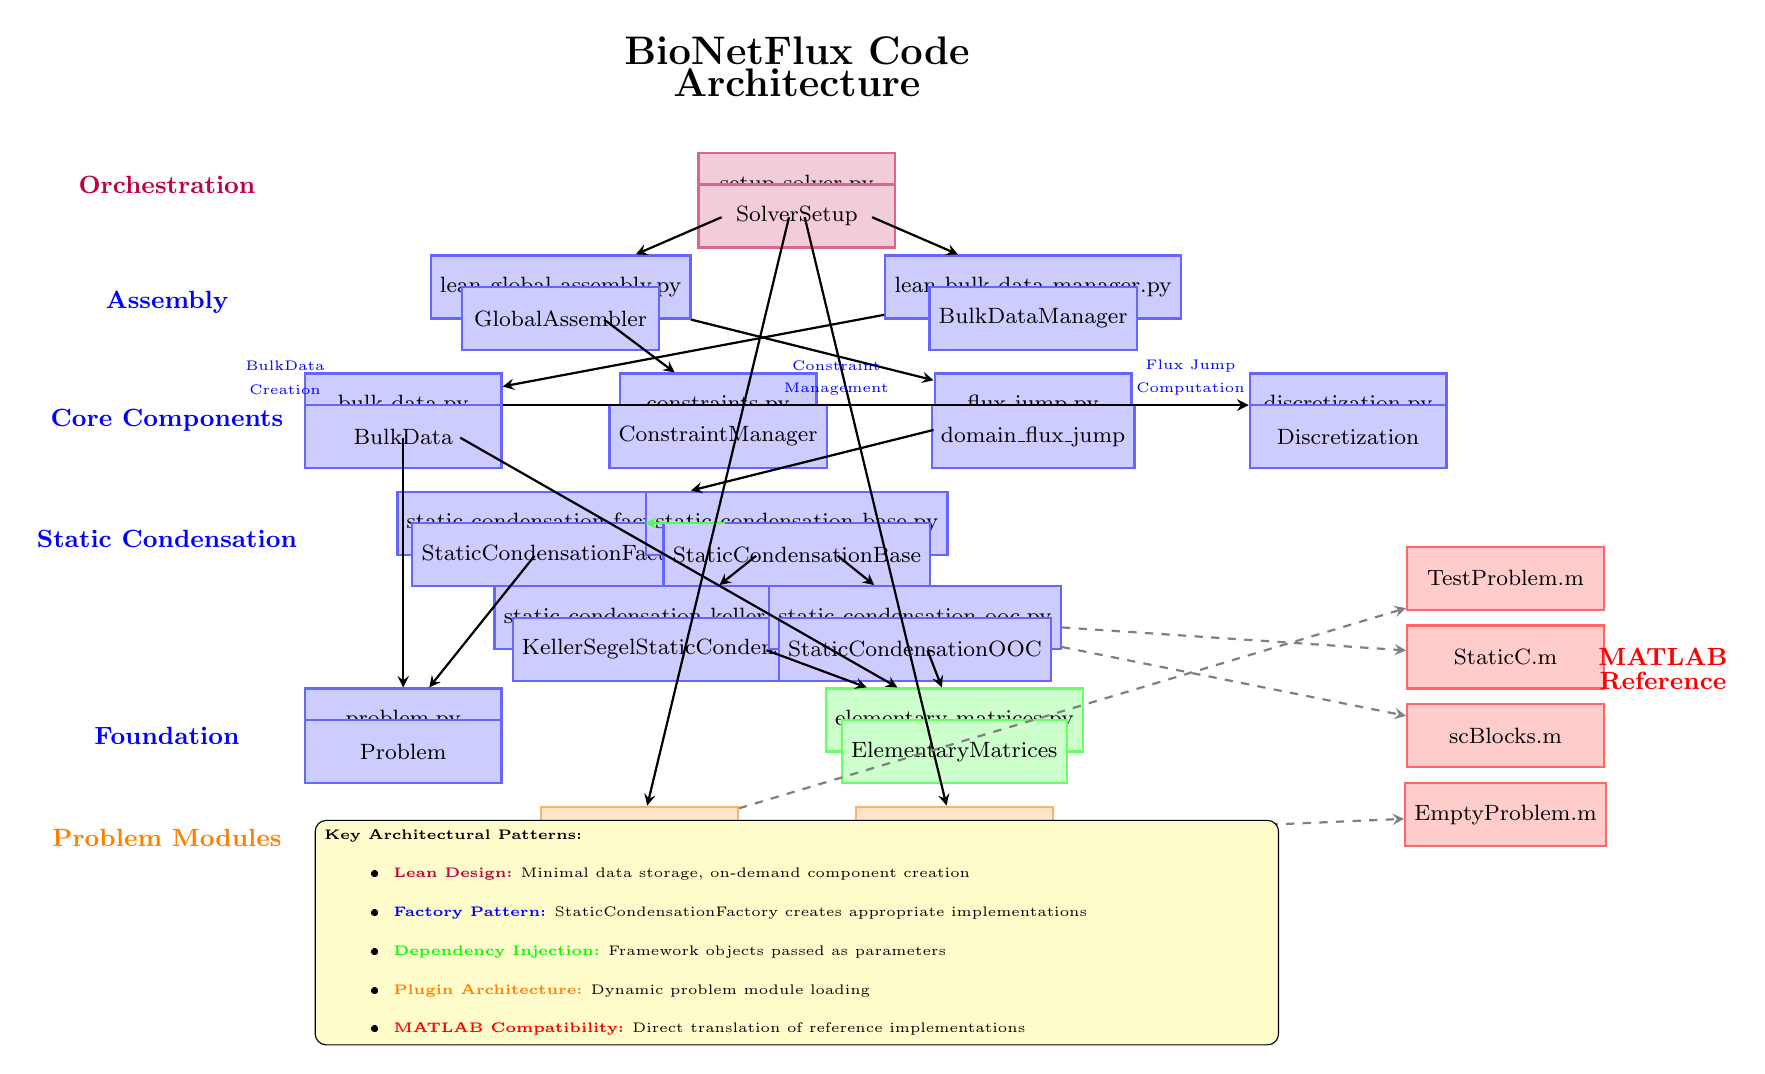
\begin{tikzpicture}[
    % Define styles
    core/.style={rectangle, draw=blue!60, fill=blue!20, thick, minimum width=2.5cm, minimum height=0.8cm, text centered, font=\footnotesize},
    utils/.style={rectangle, draw=green!60, fill=green!20, thick, minimum width=2.5cm, minimum height=0.8cm, text centered, font=\footnotesize},
    problems/.style={rectangle, draw=orange!60, fill=orange!20, thick, minimum width=2.5cm, minimum height=0.8cm, text centered, font=\footnotesize},
    setup/.style={rectangle, draw=purple!60, fill=purple!20, thick, minimum width=2.5cm, minimum height=0.8cm, text centered, font=\footnotesize},
    matlab/.style={rectangle, draw=red!60, fill=red!20, thick, minimum width=2.5cm, minimum height=0.8cm, text centered, font=\footnotesize},
    arrow/.style={->, thick, >=stealth},
    depends/.style={->, dashed, thick, >=stealth, color=gray},
    dataflow/.style={->, thick, >=stealth, color=blue!70},
    factory/.style={->, thick, >=stealth, color=green!70}
]

% Title - Split into two nodes
\node[font=\Large\bfseries] at (0, 10.2) {BioNetFlux Code};
\node[font=\Large\bfseries] at (0, 9.8) {Architecture};

% Layer 1: Setup and Orchestration (Top)
\node[setup] (setup_solver) at (0, 8.5) {setup\_solver.py};
\node[setup] (setup_solver_class) at (0, 8.1) {SolverSetup};

% Layer 2: Core Assembly (Upper Middle)
\node[core] (global_assembly) at (-3, 7.2) {lean\_global\_assembly.py};
\node[core] (global_assembly_class) at (-3, 6.8) {GlobalAssembler};
\node[core] (bulk_manager) at (3, 7.2) {lean\_bulk\_data\_manager.py};
\node[core] (bulk_manager_class) at (3, 6.8) {BulkDataManager};

% Layer 3: Core Components (Middle)
\node[core] (bulk_data) at (-5, 5.7) {bulk\_data.py};
\node[core] (bulk_data_class) at (-5, 5.3) {BulkData};
\node[core] (constraints) at (-1, 5.7) {constraints.py};
\node[core] (constraints_class) at (-1, 5.3) {ConstraintManager};
\node[core] (flux_jump) at (3, 5.7) {flux\_jump.py};
\node[core] (flux_jump_func) at (3, 5.3) {domain\_flux\_jump};
\node[core] (discretization) at (7, 5.7) {discretization.py};
\node[core] (discretization_class) at (7, 5.3) {Discretization};

% Layer 4: Static Condensation (Lower Middle)
\node[core] (sc_factory) at (-3, 4.2) {static\_condensation\_factory.py};
\node[core] (sc_factory_class) at (-3, 3.8) {StaticCondensationFactory};
\node[core] (sc_base) at (0, 4.2) {static\_condensation\_base.py};
\node[core] (sc_base_class) at (0, 3.8) {StaticCondensationBase};
\node[core] (sc_ks) at (-1.5, 3) {static\_condensation\_keller\_segel.py};
\node[core] (sc_ks_class) at (-1.5, 2.6) {KellerSegelStaticCondensation};
\node[core] (sc_ooc) at (1.5, 3) {static\_condensation\_ooc.py};
\node[core] (sc_ooc_class) at (1.5, 2.6) {StaticCondensationOOC};

% Layer 5: Foundation (Bottom)
\node[core] (problem) at (-5, 1.7) {problem.py};
\node[core] (problem_class) at (-5, 1.3) {Problem};
\node[utils] (elementary) at (2, 1.7) {elementary\_matrices.py};
\node[utils] (elementary_class) at (2, 1.3) {ElementaryMatrices};
\node[problems] (test_problem) at (-2, 0.2) {test\_problem2.py};
\node[problems] (double_arc) at (2, 0.2) {double\_arc.py};

% Layer 6: MATLAB Reference (Side)
\node[matlab] (matlab_test) at (9, 3.5) {TestProblem.m};
\node[matlab] (matlab_static) at (9, 2.5) {StaticC.m};
\node[matlab] (matlab_blocks) at (9, 1.5) {scBlocks.m};
\node[matlab] (matlab_empty) at (9, 0.5) {EmptyProblem.m};

% Main orchestration flow
\draw[arrow] (setup_solver) -- (global_assembly);
\draw[arrow] (setup_solver) -- (bulk_manager);

% Assembly dependencies
\draw[arrow] (global_assembly) -- (flux_jump);
\draw[arrow] (global_assembly) -- (constraints);
\draw[arrow] (bulk_manager) -- (bulk_data);

% Core component relationships
\draw[arrow] (flux_jump) -- (sc_factory);
\draw[arrow] (bulk_data) -- (elementary);
\draw[arrow] (bulk_data) -- (discretization);
\draw[arrow] (constraints) -- (discretization);

% Static condensation hierarchy
\draw[factory] (sc_factory) -- (sc_base);
\draw[arrow] (sc_base) -- (sc_ks);
\draw[arrow] (sc_base) -- (sc_ooc);
\draw[arrow] (sc_ks) -- (elementary);
\draw[arrow] (sc_ooc) -- (elementary);

% Problem dependencies
\draw[arrow] (bulk_data) -- (problem);
\draw[arrow] (sc_factory) -- (problem);
\draw[arrow] (setup_solver) -- (test_problem);
\draw[arrow] (setup_solver) -- (double_arc);

% MATLAB reference connections
\draw[depends] (sc_ooc) -- (matlab_static);
\draw[depends] (sc_ooc) -- (matlab_blocks);
\draw[depends] (test_problem) -- (matlab_test);
\draw[depends] (double_arc) -- (matlab_empty);

% Data flow annotations
\node[font=\tiny, color=blue] at (-6.5, 6.2) {BulkData};
\node[font=\tiny, color=blue] at (-6.5, 5.9) {Creation};
\node[font=\tiny, color=blue] at (0.5, 6.2) {Constraint};
\node[font=\tiny, color=blue] at (0.5, 5.9) {Management};
\node[font=\tiny, color=blue] at (5, 6.2) {Flux Jump};
\node[font=\tiny, color=blue] at (5, 5.9) {Computation};

% Layer labels
\node[font=\small\bfseries, color=purple] at (-8, 8.5) {Orchestration};
\node[font=\small\bfseries, color=blue] at (-8, 7) {Assembly};
\node[font=\small\bfseries, color=blue] at (-8, 5.5) {Core Components};
\node[font=\small\bfseries, color=blue] at (-8, 4) {Static Condensation};
\node[font=\small\bfseries, color=blue] at (-8, 1.5) {Foundation};
\node[font=\small\bfseries, color=orange] at (-8, 0.2) {Problem Modules};
\node[font=\small\bfseries, color=red] at (11, 2.5) {MATLAB};
\node[font=\small\bfseries, color=red] at (11, 2.2) {Reference};

% Key architectural patterns
\node[draw, rounded corners, fill=yellow!20, font=\tiny] at (0, -1) {
    \begin{minipage}{12cm}
    \textbf{Key Architectural Patterns:}
    \begin{itemize}
        \item \textcolor{purple}{\textbf{Lean Design:}} Minimal data storage, on-demand component creation
        \item \textcolor{blue}{\textbf{Factory Pattern:}} StaticCondensationFactory creates appropriate implementations
        \item \textcolor{green}{\textbf{Dependency Injection:}} Framework objects passed as parameters
        \item \textcolor{orange}{\textbf{Plugin Architecture:}} Dynamic problem module loading
        \item \textcolor{red}{\textbf{MATLAB Compatibility:}} Direct translation of reference implementations
    \end{itemize}
    \end{minipage}
};

\end{tikzpicture}
\caption[BioNetFlux Code Architecture]{
BioNetFlux code architecture showing the hierarchical structure and dependencies between modules. 
\textcolor{purple}{Purple boxes} represent orchestration layers, 
\textcolor{blue}{blue boxes} represent core computational components, 
\textcolor{green}{green boxes} represent utilities, 
\textcolor{orange}{orange boxes} represent problem-specific modules, and 
\textcolor{red}{red boxes} represent MATLAB reference implementations. 
Solid arrows indicate direct dependencies, dashed arrows indicate reference relationships, 
and colored arrows highlight specific architectural patterns (factory creation, data flow).
The lean design minimizes memory usage through on-demand component creation and parameter-based framework object passing.
}
\label{fig:bionetflux_architecture}
\end{figure}

% Supplementary detailed component diagram
\begin{figure}[htbp]
\centering
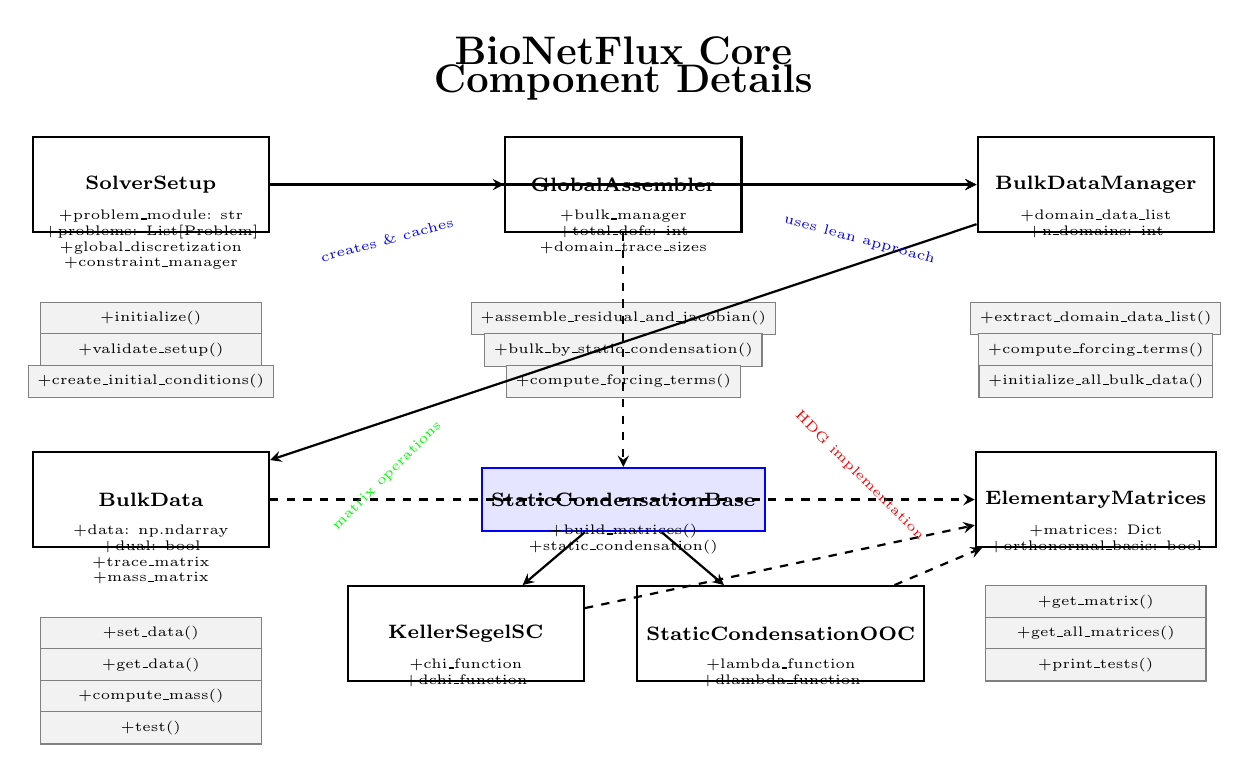
\begin{tikzpicture}[
    % Define styles - Fixed arrow tips
    class/.style={rectangle, draw=black, fill=white, thick, minimum width=3cm, minimum height=1.2cm, text centered, font=\scriptsize},
    method/.style={rectangle, draw=gray, fill=gray!10, minimum width=2.8cm, minimum height=0.4cm, text centered, font=\tiny},
    interface/.style={rectangle, draw=blue, fill=blue!10, thick, minimum width=3cm, minimum height=0.8cm, text centered, font=\scriptsize},
    composition/.style={->, thick, >=stealth},
    inheritance/.style={->, thick, >=stealth},
    usage/.style={->, dashed, thick, >=stealth}
]

% Title
\node[font=\Large\bfseries] at (0, 8.2) {BioNetFlux Core};
\node[font=\Large\bfseries] at (0, 7.8) {Component Details};

% SolverSetup detail
\node[class] (setup_detail) at (-6, 6.5) {
    \textbf{SolverSetup}
};
\node[font=\tiny] at (-6, 6.1) {+problem\_module: str};
\node[font=\tiny] at (-6, 5.9) {+problems: List[Problem]};
\node[font=\tiny] at (-6, 5.7) {+global\_discretization};
\node[font=\tiny] at (-6, 5.5) {+constraint\_manager};

\node[method] (setup_methods) at (-6, 4.8) {+initialize()};
\node[method] (setup_methods2) at (-6, 4.4) {+validate\_setup()};
\node[method] (setup_methods3) at (-6, 4.0) {+create\_initial\_conditions()};

% GlobalAssembler detail
\node[class] (assembler_detail) at (0, 6.5) {
    \textbf{GlobalAssembler}
};
\node[font=\tiny] at (0, 6.1) {+bulk\_manager};
\node[font=\tiny] at (0, 5.9) {+total\_dofs: int};
\node[font=\tiny] at (0, 5.7) {+domain\_trace\_sizes};

\node[method] (assembler_methods) at (0, 4.8) {+assemble\_residual\_and\_jacobian()};
\node[method] (assembler_methods2) at (0, 4.4) {+bulk\_by\_static\_condensation()};
\node[method] (assembler_methods3) at (0, 4.0) {+compute\_forcing\_terms()};

% BulkDataManager detail
\node[class] (manager_detail) at (6, 6.5) {
    \textbf{BulkDataManager}
};
\node[font=\tiny] at (6, 6.1) {+domain\_data\_list};
\node[font=\tiny] at (6, 5.9) {+n\_domains: int};

\node[method] (manager_methods) at (6, 4.8) {+extract\_domain\_data\_list()};
\node[method] (manager_methods2) at (6, 4.4) {+compute\_forcing\_terms()};
\node[method] (manager_methods3) at (6, 4.0) {+initialize\_all\_bulk\_data()};

% BulkData detail
\node[class] (bulk_detail) at (-6, 2.5) {
    \textbf{BulkData}
};
\node[font=\tiny] at (-6, 2.1) {+data: np.ndarray};
\node[font=\tiny] at (-6, 1.9) {+dual: bool};
\node[font=\tiny] at (-6, 1.7) {+trace\_matrix};
\node[font=\tiny] at (-6, 1.5) {+mass\_matrix};

\node[method] (bulk_methods) at (-6, 0.8) {+set\_data()};
\node[method] (bulk_methods2) at (-6, 0.4) {+get\_data()};
\node[method] (bulk_methods3) at (-6, 0.0) {+compute\_mass()};
\node[method] (bulk_methods4) at (-6, -0.4) {+test()};

% StaticCondensation hierarchy
\node[interface] (sc_interface) at (0, 2.5) {
    \textbf{StaticCondensationBase}
};
\node[font=\tiny] at (0, 2.1) {+build\_matrices()};
\node[font=\tiny] at (0, 1.9) {+static\_condensation()};

\node[class] (sc_ks_detail) at (-2, 0.8) {
    \textbf{KellerSegelSC}
};
\node[font=\tiny] at (-2, 0.4) {+chi\_function};
\node[font=\tiny] at (-2, 0.2) {+dchi\_function};

\node[class] (sc_ooc_detail) at (2, 0.8) {
    \textbf{StaticCondensationOOC}
};
\node[font=\tiny] at (2, 0.4) {+lambda\_function};
\node[font=\tiny] at (2, 0.2) {+dlambda\_function};

% ElementaryMatrices detail
\node[class] (elem_detail) at (6, 2.5) {
    \textbf{ElementaryMatrices}
};
\node[font=\tiny] at (6, 2.1) {+matrices: Dict};
\node[font=\tiny] at (6, 1.9) {+orthonormal\_basis: bool};

\node[method] (elem_methods) at (6, 1.2) {+get\_matrix()};
\node[method] (elem_methods2) at (6, 0.8) {+get\_all\_matrices()};
\node[method] (elem_methods3) at (6, 0.4) {+print\_tests()};

% Relationships - Using stealth arrow tips for all
\draw[composition] (setup_detail) -- (assembler_detail);
\draw[composition] (setup_detail) -- (manager_detail);
\draw[composition] (assembler_detail) -- (manager_detail);
\draw[composition] (manager_detail) -- (bulk_detail);
\draw[usage] (assembler_detail) -- (sc_interface);
\draw[inheritance] (sc_interface) -- (sc_ks_detail);
\draw[inheritance] (sc_interface) -- (sc_ooc_detail);
\draw[usage] (bulk_detail) -- (elem_detail);
\draw[usage] (sc_ks_detail) -- (elem_detail);
\draw[usage] (sc_ooc_detail) -- (elem_detail);

% Data flow indicators
\node[font=\tiny, color=blue, rotate=15] at (-3, 5.8) {creates \& caches};
\node[font=\tiny, color=blue, rotate=-15] at (3, 5.8) {uses lean approach};
\node[font=\tiny, color=green, rotate=45] at (-3, 2.8) {matrix operations};
\node[font=\tiny, color=red, rotate=-45] at (3, 2.8) {HDG implementation};

\end{tikzpicture}
\caption[BioNetFlux Component Details]{
Detailed view of key BioNetFlux components showing class structures, main attributes, and key methods. 
Solid arrows indicate composition and inheritance relationships, 
and dashed arrows represent usage dependencies. 
The diagram emphasizes the lean design pattern where components are created on-demand and cached for efficiency.
}
\label{fig:bionetflux_components}
\end{figure}

% Data flow diagram
\begin{figure}[htbp]
\centering
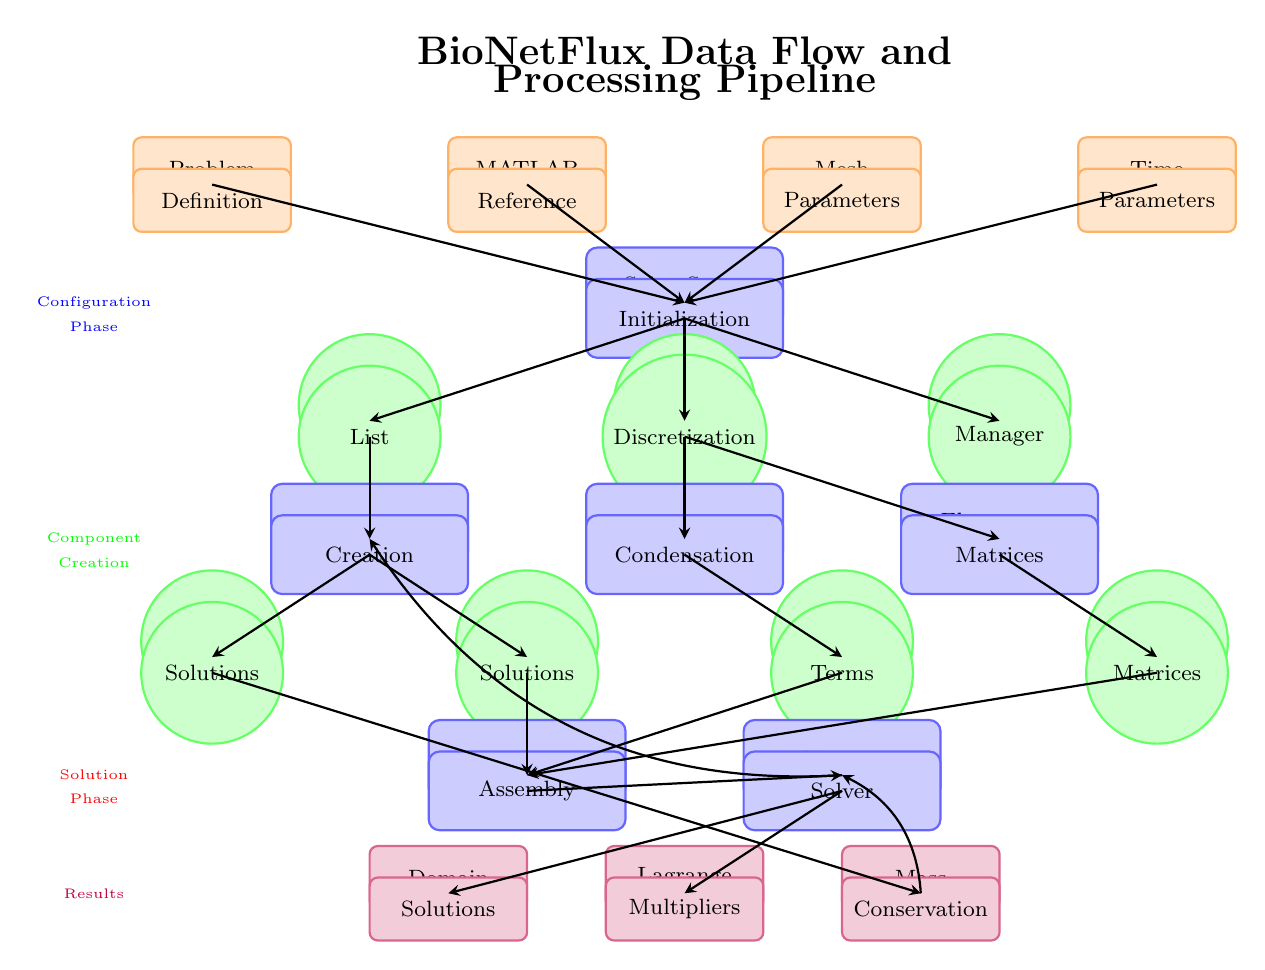
\begin{tikzpicture}[
    % Define styles - Fixed shapes using basic rectangles and circles
    process/.style={rectangle, rounded corners, draw=blue!60, fill=blue!20, thick, minimum width=2.5cm, minimum height=1cm, text centered, font=\footnotesize},
    data/.style={circle, draw=green!60, fill=green!20, thick, minimum width=1.8cm, text centered, font=\footnotesize},
    input/.style={rectangle, rounded corners=3pt, draw=orange!60, fill=orange!20, thick, minimum width=2cm, minimum height=0.8cm, text centered, font=\footnotesize},
    output/.style={rectangle, rounded corners=3pt, draw=purple!60, fill=purple!20, thick, minimum width=2cm, minimum height=0.8cm, text centered, font=\footnotesize},
    flow/.style={->, thick, >=stealth}
]

% Title
\node[font=\Large\bfseries] at (0, 9.2) {BioNetFlux Data Flow and};
\node[font=\Large\bfseries] at (0, 8.8) {Processing Pipeline};

% Input layer
\node[input] (problem_def_top) at (-6, 7.7) {Problem};
\node[input] (problem_def_bot) at (-6, 7.3) {Definition};
\node[input] (matlab_ref_top) at (-2, 7.7) {MATLAB};
\node[input] (matlab_ref_bot) at (-2, 7.3) {Reference};
\node[input] (mesh_params_top) at (2, 7.7) {Mesh};
\node[input] (mesh_params_bot) at (2, 7.3) {Parameters};
\node[input] (time_params_top) at (6, 7.7) {Time};
\node[input] (time_params_bot) at (6, 7.3) {Parameters};

% Processing layer 1: Setup
\node[process] (setup_process_top) at (0, 6.2) {SolverSetup};
\node[process] (setup_process_bot) at (0, 5.8) {Initialization};

% Data layer 1
\node[data] (problems_data_top) at (-4, 4.7) {Problems};
\node[data] (problems_data_bot) at (-4, 4.3) {List};
\node[data] (discretization_data_top) at (0, 4.7) {Global};
\node[data] (discretization_data_bot) at (0, 4.3) {Discretization};
\node[data] (constraints_data_top) at (4, 4.7) {Constraint};
\node[data] (constraints_data_bot) at (4, 4.3) {Manager};

% Processing layer 2: Component Creation
\node[process] (bulk_creation_top) at (-4, 3.2) {BulkData};
\node[process] (bulk_creation_bot) at (-4, 2.8) {Creation};
\node[process] (sc_creation_top) at (0, 3.2) {Static};
\node[process] (sc_creation_bot) at (0, 2.8) {Condensation};
\node[process] (matrix_creation_top) at (4, 3.2) {Elementary};
\node[process] (matrix_creation_bot) at (4, 2.8) {Matrices};

% Data layer 2
\node[data] (bulk_solutions_top) at (-6, 1.7) {Bulk};
\node[data] (bulk_solutions_bot) at (-6, 1.3) {Solutions};
\node[data] (trace_solutions_top) at (-2, 1.7) {Trace};
\node[data] (trace_solutions_bot) at (-2, 1.3) {Solutions};
\node[data] (forcing_terms_top) at (2, 1.7) {Forcing};
\node[data] (forcing_terms_bot) at (2, 1.3) {Terms};
\node[data] (matrices_top) at (6, 1.7) {System};
\node[data] (matrices_bot) at (6, 1.3) {Matrices};

% Processing layer 3: Assembly and Solving
\node[process] (assembly_process_top) at (-2, 0.2) {Global};
\node[process] (assembly_process_bot) at (-2, -0.2) {Assembly};
\node[process] (newton_process_top) at (2, 0.2) {Newton};
\node[process] (newton_process_bot) at (2, -0.2) {Solver};

% Output layer
\node[output] (solution_output_top) at (-3, -1.3) {Domain};
\node[output] (solution_output_bot) at (-3, -1.7) {Solutions};
\node[output] (multiplier_output_top) at (0, -1.3) {Lagrange};
\node[output] (multiplier_output_bot) at (0, -1.7) {Multipliers};
\node[output] (conservation_output_top) at (3, -1.3) {Mass};
\node[output] (conservation_output_bot) at (3, -1.7) {Conservation};

% Flow connections (connecting to center points)
\draw[flow] (-6, 7.5) -- (0, 6);
\draw[flow] (-2, 7.5) -- (0, 6);
\draw[flow] (2, 7.5) -- (0, 6);
\draw[flow] (6, 7.5) -- (0, 6);

\draw[flow] (0, 5.8) -- (-4, 4.5);
\draw[flow] (0, 5.8) -- (0, 4.5);
\draw[flow] (0, 5.8) -- (4, 4.5);

\draw[flow] (-4, 4.3) -- (-4, 3);
\draw[flow] (0, 4.3) -- (0, 3);
\draw[flow] (0, 4.3) -- (4, 3);

\draw[flow] (-4, 2.8) -- (-6, 1.5);
\draw[flow] (-4, 2.8) -- (-2, 1.5);
\draw[flow] (0, 2.8) -- (2, 1.5);
\draw[flow] (4, 2.8) -- (6, 1.5);

\draw[flow] (-2, 1.3) -- (-2, 0);
\draw[flow] (2, 1.3) -- (-2, 0);
\draw[flow] (6, 1.3) -- (-2, 0);
\draw[flow] (-2, -0.2) -- (2, 0);

\draw[flow] (2, -0.2) -- (-3, -1.5);
\draw[flow] (2, -0.2) -- (0, -1.5);
\draw[flow] (-6, 1.3) -- (3, -1.5);

% Feedback loops
\draw[flow, bend left=30] (2, 0) to (-4, 3);
\draw[flow, bend right=30] (3, -1.5) to (2, 0);

% Annotations
\node[font=\tiny, color=blue] at (-7.5, 6) {Configuration};
\node[font=\tiny, color=blue] at (-7.5, 5.7) {Phase};
\node[font=\tiny, color=green] at (-7.5, 3) {Component};
\node[font=\tiny, color=green] at (-7.5, 2.7) {Creation};
\node[font=\tiny, color=red] at (-7.5, 0) {Solution};
\node[font=\tiny, color=red] at (-7.5, -0.3) {Phase};
\node[font=\tiny, color=purple] at (-7.5, -1.5) {Results};

\end{tikzpicture}
\caption[BioNetFlux Data Flow]{
BioNetFlux data flow and processing pipeline showing the transformation from input parameters through component creation to final solutions. 
Orange rectangles represent input data, blue rounded rectangles represent processing steps, 
green circles represent intermediate data structures, and purple rectangles represent outputs. 
The diagram illustrates the lean approach where components are created on-demand and data flows efficiently through the processing pipeline.
Feedback loops show the iterative nature of the Newton solver and mass conservation monitoring.
}
\label{fig:bionetflux_dataflow}
\end{figure}
